\documentclass[11pt,letterpaper]{article}
\usepackage[utf8]{inputenc}
\usepackage[T1]{fontenc}
\usepackage[spanish]{babel}
\usepackage{amsmath,amssymb}
\usepackage{graphicx}
\usepackage{float}
\usepackage{url}
\usepackage{tikz}
\usepackage{pgfplots}
\pgfplotsset{compat=1.18}
\usetikzlibrary{arrows.meta,calc,positioning,babel}
\graphicspath{{figuras/}}

\newcommand{\naglecite}[1]{\emph{(véase Nagle, #1)}}

\begin{document}

\textbf{3 de Junio}

\[
\vec{X}' = A\vec{X}, \qquad A \in M_{n\times n}(\mathbb{R})
\]

\[
\lambda \in \mathbb{R}, \qquad v \in \mathbb{R}^n, \qquad X:\mathbb{R}\to\mathbb{R}^n
\]

\[
X(t)=e^{\lambda t}v
\]

\[
\begin{cases}
x_1' = a_{11}x_1 + \cdots + a_{1n}x_n\\
\vdots\\
x_n' = a_{n1}x_1 + \cdots + a_{nn}x_n
\end{cases}
\]

\[
x' = ax \Rightarrow x(t)=x_0e^{at}, \qquad x_0=x(0)
\]

\[
X(t)\ \text{puede tener solucion?}
\]

\[
X'(t)=\lambda e^{\lambda t}v
\]

\[
X(t)\ \text{es solucion si}
\]

\[
\lambda e^{\lambda t}v=e^{\lambda t}Av
\]

\[
\Rightarrow Av=\lambda v
\]

\[
X(t)=e^{\lambda t}v\ \text{es solucion si } \lambda \text{ es valor propio de } A \text{ y } v \text{ es su correspondiente vector propio}
\]

\[
\text{Si } A \text{ tiene } n \text{ valores propios distintos } \lambda_1,\lambda_2,\ldots,\lambda_n
\]

\[
\text{y sus correspondientes vectores propios } v_1,\ldots,v_n
\]

\[
\text{estos son linealmente independientes}
\]

\[
\Rightarrow \left\{X_j(t)=e^{\lambda_j t}v_j\right\}_{j=1}^n
\]

\[
\text{en un conjunto de soluciones linealmente independientes}
\]

\newpage

\textbf{Captura 02}

\[
\text{Referencias: Devaney, Hirsch, Smale.}
\]

\[
\text{Teoria de ecuaciones diferenciales, sistemas dinamicos, Arrowsmith y Place.}
\]

\[
x' = F(x), \qquad F:\mathbb{R}^n\to\mathbb{R}^n,\qquad F\in C^1
\]

\[
\text{Problema general: estudiar la din\'amica global de las soluciones de }(*)
\]

\[
\text{Din\'amica local: dado } x_0\in\mathbb{R}^n,\ \text{¿cu\'al es el comportamiento de las soluciones cerca de }x_0?
\]

\[
\text{Posibilidades}
\]

\[
1)\ x_0 \text{ en un punto regular}, \qquad F(x_0)\neq \vec 0.
\]

\[
2)\ x_0 \text{ es un punto de equilibrio}, \qquad F(x_0)=\vec 0.
\]

\begin{figure}[H]
\centering
\begin{tikzpicture}[scale=0.95,>=Stealth]
  \newcommand{\miniaxes}{
    \draw[->] (-1.4,0) -- (1.4,0);
    \draw[->] (0,-1.4) -- (0,1.4);
  }

  \begin{scope}[shift={(-4.3,2.0)}]
    \miniaxes
    \foreach \a in {0,30,...,330} {
      \draw[blue!70,->,line width=0.35pt] (0,0) -- ({1.05*cos(\a)},{1.05*sin(\a)});
    }
    \node[font=\small] at (0,-1.85) {Fuente};
  \end{scope}

  \begin{scope}[shift={(0,2.0)}]
    \miniaxes
    \foreach \a in {0,30,...,330} {
      \draw[blue!70,->,line width=0.35pt] ({1.05*cos(\a)},{1.05*sin(\a)}) -- (0,0);
    }
    \node[font=\small] at (0,-1.85) {Sumidero};
  \end{scope}

  \begin{scope}[shift={(4.3,2.0)}]
    \miniaxes
    \draw[red!75,->,line width=0.45pt] (-1.2,0) -- (-0.15,0);
    \draw[red!75,->,line width=0.45pt] (0.15,0) -- (1.2,0);
    \draw[blue!70,->,line width=0.45pt] (0,-1.2) -- (0,-0.15);
    \draw[blue!70,->,line width=0.45pt] (0,1.2) -- (0,0.15);
    \draw[blue!70,thick] plot[domain=-1.2:-0.25,samples=70] (\x,{0.65/\x});
    \draw[blue!70,thick] plot[domain=0.25:1.2,samples=70] (\x,{0.65/\x});
    \draw[blue!70,thick] plot[domain=-1.2:-0.25,samples=70] (\x,{-0.65/\x});
    \draw[blue!70,thick] plot[domain=0.25:1.2,samples=70] (\x,{-0.65/\x});
    \node[font=\small] at (0,-1.85) {Silla};
  \end{scope}

  \begin{scope}[shift={(-2.15,-2.4)}]
    \miniaxes
    \draw[blue!70,->,line width=0.5pt,domain=0:5.6,samples=150]
      plot ({0.92*exp(-0.18*\x)*cos(\x r)},{0.92*exp(-0.18*\x)*sin(\x r)});
    \node[font=\small] at (0,-1.85) {Espiral};
  \end{scope}

  \begin{scope}[shift={(2.15,-2.4)}]
    \miniaxes
    \draw[blue!70,->,line width=0.55pt] (0.78,0) arc (0:335:0.78);
    \draw[blue!70,->,line width=0.55pt] (0.50,0) arc (0:335:0.50);
    \node[font=\small] at (0,-1.85) {Centro};
  \end{scope}
\end{tikzpicture}
\caption{Esquemas locales t\'ipicos para la din\'amica en el plano.}
\end{figure}

\[
x' = f(x), \qquad f\in C^1
\]

\[
y\ x_0 \text{ es un punto de equilibrio}, \qquad F(x_0)=\vec 0
\]

\[
\text{Calculemos el jacobiano}
\]

\[
F=(F_1(x,y),F_2(x,y))
\]

\[
J(x)=
\begin{pmatrix}
\dfrac{\partial F_1}{\partial x}(x,y) & \dfrac{\partial F_1}{\partial y}(x,y)\\[1ex]
\dfrac{\partial F_2}{\partial x}(x,y) & \dfrac{\partial F_2}{\partial y}(x,y)
\end{pmatrix}
\]

\[
\text{Ejemplo de linealizaci\'on}
\]

\[
x' = x^2-y^2-1
\]

\[
y' = 2y
\]

\[
DF(x)=J(x)=
\begin{pmatrix}
2x & -2y\\
0 & 2
\end{pmatrix}
\]

\[
\text{Punto de equilibrio de (1):}\qquad x^2-y^2-1=0,\qquad 2y=0
\]

\[
\text{Como } y=0 \to x^2-1=0 \to x=\pm 1
\]

\[
\text{Tenemos dos puntos de equilibrio: } x_0=(1,0)\ \text{y}\ x_1=(-1,0)
\]

\begin{figure}[H]
\centering
\begin{tikzpicture}[scale=1.05,>=Stealth]
  \draw[->] (-2.5,0) -- (2.5,0) node[right] {$x$};
  \draw[->] (0,-2.5) -- (0,2.5) node[above] {$y$};

  \foreach \x in {-2,-1.5,...,2} {
    \foreach \y in {-2,-1.5,...,2} {
      \pgfmathsetmacro{\u}{\x*\x - \y*\y - 1}
      \pgfmathsetmacro{\v}{2*\y}
      \pgfmathsetmacro{\nrm}{max(0.35,sqrt(\u*\u+\v*\v))}
      \draw[blue!70,->,line width=0.35pt,opacity=0.9]
        (\x,\y) -- ++({0.22*\u/\nrm},{0.22*\v/\nrm});
    }
  }

  \draw[yellow!85!orange,thick] (-2.35,0) -- (2.35,0);
  \draw[orange!85!red,thick] plot[domain=1:2.25,samples=120] (\x,{sqrt(\x*\x-1)});
  \draw[orange!85!red,thick] plot[domain=1:2.25,samples=120] (\x,{-sqrt(\x*\x-1)});
  \draw[orange!85!red,thick] plot[domain=-2.25:-1,samples=120] (\x,{sqrt(\x*\x-1)});
  \draw[orange!85!red,thick] plot[domain=-2.25:-1,samples=120] (\x,{-sqrt(\x*\x-1)});

  \fill[black] (1,0) circle (0.05);
  \fill[black] (-1,0) circle (0.05);
  \node[black,below right] at (1,0) {$(1,0)$};
  \node[black,below left] at (-1,0) {$(-1,0)$};
\end{tikzpicture}
\caption{Campo vectorial esquematico del sistema $x'=x^2-y^2-1$, $y'=2y$ con sus nullclines y puntos de equilibrio.}
\end{figure}

\newpage

\textbf{Taylor de primer orden}

\[
f(x)\simeq f(x_0), \qquad \forall x\in(x_0-\varepsilon,\;x_0+\varepsilon)
\]

\[
f(x)\simeq f(x_0)+f'(x_0)(x-x_0)
\]

\[
y=f(x_0)+f'(x_0)(x-x_0)
\]

\[
f:(a,b)\to\mathbb{R}, \qquad f\in C^2
\]

\[
f(x)\simeq f(x_0)+f'(x_0)(x-x_0)+\frac12 f''(x_0)(x-x_0)^2
\]

\[
\forall x\in(x_0-\varepsilon,\;x_0+\varepsilon)
\]

\[
f(x)=\sum_{i=0}^{\infty}\frac{f^{(i)}(x_0)}{i!}(x-x_0)^i
\]

\[
=\sum_{i=0}^{n}\frac{f^{(i)}(x_0)}{i!}(x-x_0)^i+R_n(x)
\]

\begin{figure}[H]
\centering
\begin{tikzpicture}[scale=0.95]
  \begin{scope}
    \draw[->] (-0.2,0) -- (4.2,0) node[right] {$x$};
    \draw[->] (0,-0.2) -- (0,2.1) node[above] {$y$};
    \draw[red!80!black,thick] (0.5,1.2) -- (3.5,1.2);
    \draw[dashed] (1.1,0) -- (1.1,1.2);
    \draw[dashed] (2.0,0) -- (2.0,1.2);
    \draw[dashed] (2.9,0) -- (2.9,1.2);
    \node[below] at (1.1,0) {$x_0-\varepsilon$};
    \node[below] at (2.0,0) {$x_0$};
    \node[below] at (2.9,0) {$x_0+\varepsilon$};
    \node[red!80!black] at (2.0,1.55) {$f(x)\simeq f(x_0)$};
  \end{scope}
  \begin{scope}[xshift=6.0cm]
    \draw[->] (-0.2,0) -- (4.2,0) node[right] {$x$};
    \draw[->] (0,-0.2) -- (0,2.1) node[above] {$y$};
    \draw[blue!70!black,thick] plot[smooth] coordinates {(0.4,0.45) (0.9,0.78) (1.4,1.02) (1.9,1.20) (2.4,1.30) (2.9,1.42) (3.4,1.56)};
    \draw[red!80!black,thick] (0.6,0.55) -- (3.3,1.78);
    \fill (1.9,1.20) circle (0.04) node[below right] {$x_0$};
    \draw[dashed] (1.9,0) -- (1.9,1.20);
    \node[red!80!black] at (2.6,1.9) {$f(x_0)+f'(x_0)(x-x_0)$};
  \end{scope}
\end{tikzpicture}
\caption{Aproximacion de orden cero y primer orden.}
\end{figure}

\begin{figure}[H]
\centering
\begin{tikzpicture}[scale=1]
  \draw[->] (-0.2,0) -- (4.2,0) node[right] {$x$};
  \draw[->] (0,-0.2) -- (0,2.6) node[above] {$y$};
  \draw[blue!70!black,thick] plot[smooth] coordinates {(0.4,0.4) (0.9,0.75) (1.4,1.02) (1.9,1.25) (2.4,1.42) (2.9,1.50) (3.4,1.58)};
  \draw[red!80!black,thick] plot[smooth] coordinates {(0.4,0.55) (0.9,0.82) (1.4,1.03) (1.9,1.23) (2.4,1.40) (2.9,1.55) (3.4,1.72)};
  \fill (1.9,1.25) circle (0.04) node[below right] {$x_0$};
  \draw[dashed] (1.9,0) -- (1.9,1.25);
  \node[red!80!black] at (2.8,2.15) {$f(x)\simeq f(x_0)+f'(x_0)(x-x_0)+\frac12 f''(x_0)(x-x_0)^2$};
\end{tikzpicture}
\caption{Aproximacion de segundo orden.}
\end{figure}

\newpage

\textbf{Taylor en dimension 2}

\[
x' = F(x), \qquad x\in\mathbb{R}^n
\]

\[
F:\mathbb{R}^n\to\mathbb{R}^n, \qquad \text{campo vectorial de clase } C^\infty
\]

\[
F=(F_1,F_2)
\]

\[
\text{Tomemos }x_0=(x_0,y_0)\in\mathbb{R}^2,\qquad x=(x,y)
\]

\[
h=x-x_0,\qquad k=y-y_0
\]

\[
F(x_0+h,y_0+k)=F(x_0,y_0)+DF(x_0,y_0)\binom{h}{k}+\frac12\binom{a_1(h,k)}{a_2(h,k)}
\]

\[
DF(x_0,y_0)=J(x_0,y_0)=
\begin{pmatrix}
\dfrac{\partial F_1}{\partial x}(x_0,y_0) & \dfrac{\partial F_1}{\partial y}(x_0,y_0)\\[1ex]
\dfrac{\partial F_2}{\partial x}(x_0,y_0) & \dfrac{\partial F_2}{\partial y}(x_0,y_0)
\end{pmatrix}
\]

\[
\text{Uno quisiera que la primera aproximacion de }F\text{ nos de informacion en una vecindad de }x_0
\]

\[
\text{si es un punto de equilibrio}
\]

\[
X=(x,y)\sim X_0=(x_0,y_0)
\]

\[
F(X)\simeq F(X_0)+DF(X_0)\binom{h}{k}
\]

\[
Y'=DF(X_0)Y, \qquad DF(X_0)=A\in M_{2\times 2}(\mathbb{R})
\]

\[
Y'=AY
\]

\[
\text{Como es el comportamiento de las soluciones de }x'=F(x)\text{ cerca de }x_0\text{ en un punto de equilibrio?}
\]

\begin{figure}[H]
\centering
\begin{tikzpicture}[scale=1]
  \draw[->] (-0.2,0) -- (4.8,0) node[right] {$x$};
  \draw[->] (0,-0.2) -- (0,4.0) node[above] {$y$};
  \draw[dashed,gray] (1.4,2.0) circle (1.1);
  \fill (1.4,2.0) circle (0.05) node[above right] {$x_0$};
  \draw[->,thick] (1.4,2.0) -- (2.2,2.45) node[midway,above] {$h$};
  \fill (2.2,2.45) circle (0.04) node[right] {$x_0+h$};
  \node at (3.15,3.05) {$F(x_0+h)\simeq F(x_0)+DF(x_0)h$};
\end{tikzpicture}
\caption{Esquema de linealizacion local alrededor de un punto.}
\end{figure}

\newpage

\underline{\textbf{Teorema de Hartman-Grobman}}

\[
\text{Sea } X'=F(X) \text{ un sistema en } \mathbb{R}^n \text{ de clase } C^1,
\]

\[
\text{definido en } \Omega\subseteq \mathbb{R}^n \text{ abierto, y } x_0 \text{ un punto de equilibrio.}
\]

\[
\text{Decimos que } x_0 \text{ es hiperb\'olico si los valores propios de } DF(x_0)
\text{ no tienen parte real nula.}
\]

\[
\text{Para } X'=F(X),\ F\in C^1(\Omega,\mathbb{R}^n),\ \text{con } x_0 \text{ un punto de equilibrio hiperb\'olico,}
\]

\[
\text{existen}
\]

\begin{itemize}
\item[(i)] vecindades \(U_{x_0}\subset \Omega\) y \(V_0\subset \mathbb{R}^n\),
\item[(ii)] una conjugaci\'on topol\'ogica local \(H:U_{x_0}\to V_0\) tal que
\end{itemize}

\[
H(\varphi_t(x))=\psi_t(H(x)).
\]

\begin{figure}[H]
\centering
\begin{tikzpicture}[>=Latex, scale=1]
  \begin{scope}[xshift=-4.6cm, yshift=0.8cm]
    \node[red!70!black] at (1.25,1.95) {$X'=F(X)$};
    \draw[->,gray!80] (0.0,0.0) -- (2.6,0.0) node[right] {$\mathbb{R}^n$};
    \draw[->,gray!80] (0.0,0.0) -- (0.0,2.4);
    \fill (1.25,1.05) circle (0.04) node[below left] {$x_0$};
    \draw[dashed,red!55] (1.25,1.05) circle (0.62);
    \node[red!55] at (1.28,0.18) {$U_{x_0}$};
    \draw[very thick,blue!70!black,->] (0.92,1.42) .. controls (1.00,1.78) and (1.32,1.70) .. (1.55,1.34);
    \node at (1.86,1.52) {$\varphi_t(x)$};
  \end{scope}

  \begin{scope}[xshift=4.6cm, yshift=0.8cm]
    \node[red!70!black] at (1.25,1.95) {$Y'=DF(x_0)Y$};
    \draw[->,gray!80] (0.0,0.0) -- (2.6,0.0) node[right] {$\mathbb{R}^n$};
    \draw[->,gray!80] (0.0,0.0) -- (0.0,2.4);
    \fill (1.25,1.05) circle (0.04) node[below left] {$H(x_0)$};
    \draw[dashed,red!55] (1.25,1.05) circle (0.62);
    \node[red!55] at (1.30,0.18) {$V_0$};
    \draw[very thick,blue!70!black,->] (0.96,1.34) .. controls (1.10,1.68) and (1.38,1.63) .. (1.58,1.30);
    \node at (1.86,1.52) {$\psi_t(H(x))$};
  \end{scope}

  \draw[->,very thick,teal!70!black] (0.85,1.85) -- node[above] {$H$} (3.15,1.85);

  \node (A) at (-3.2,-1.35) {$U_{x_0}\subset \mathbb{R}^n$};
  \node (B) at ( 3.2,-1.35) {$V_0\subset \mathbb{R}^n$};
  \node (C) at (-3.2,-3.0) {$\varphi_t(U_{x_0})\subset \mathbb{R}^n$};
  \node (D) at ( 3.2,-3.0) {$\psi_t(V_0)\subset \mathbb{R}^n$};

  \draw[->] (A) -- node[above] {$H$} (B);
  \draw[->] (A) -- node[left] {$\varphi_t$} (C);
  \draw[->] (B) -- node[right] {$\psi_t$} (D);
  \draw[->] (C) -- node[below] {$H$} (D);
\end{tikzpicture}
\caption{Esquema del teorema de Hartman-Grobman: conjugaci\'on topol\'ogica local entre el flujo no lineal y el sistema linealizado.}
\end{figure}

\[
\varphi_t \text{ es el flujo asociado a } X'=F(X), \qquad
\psi_t \text{ es el flujo asociado a } Y'=DF(x_0)Y.
\]

\textbf{Gr\'aficas asociadas al teorema}

\begin{figure}[H]
\centering
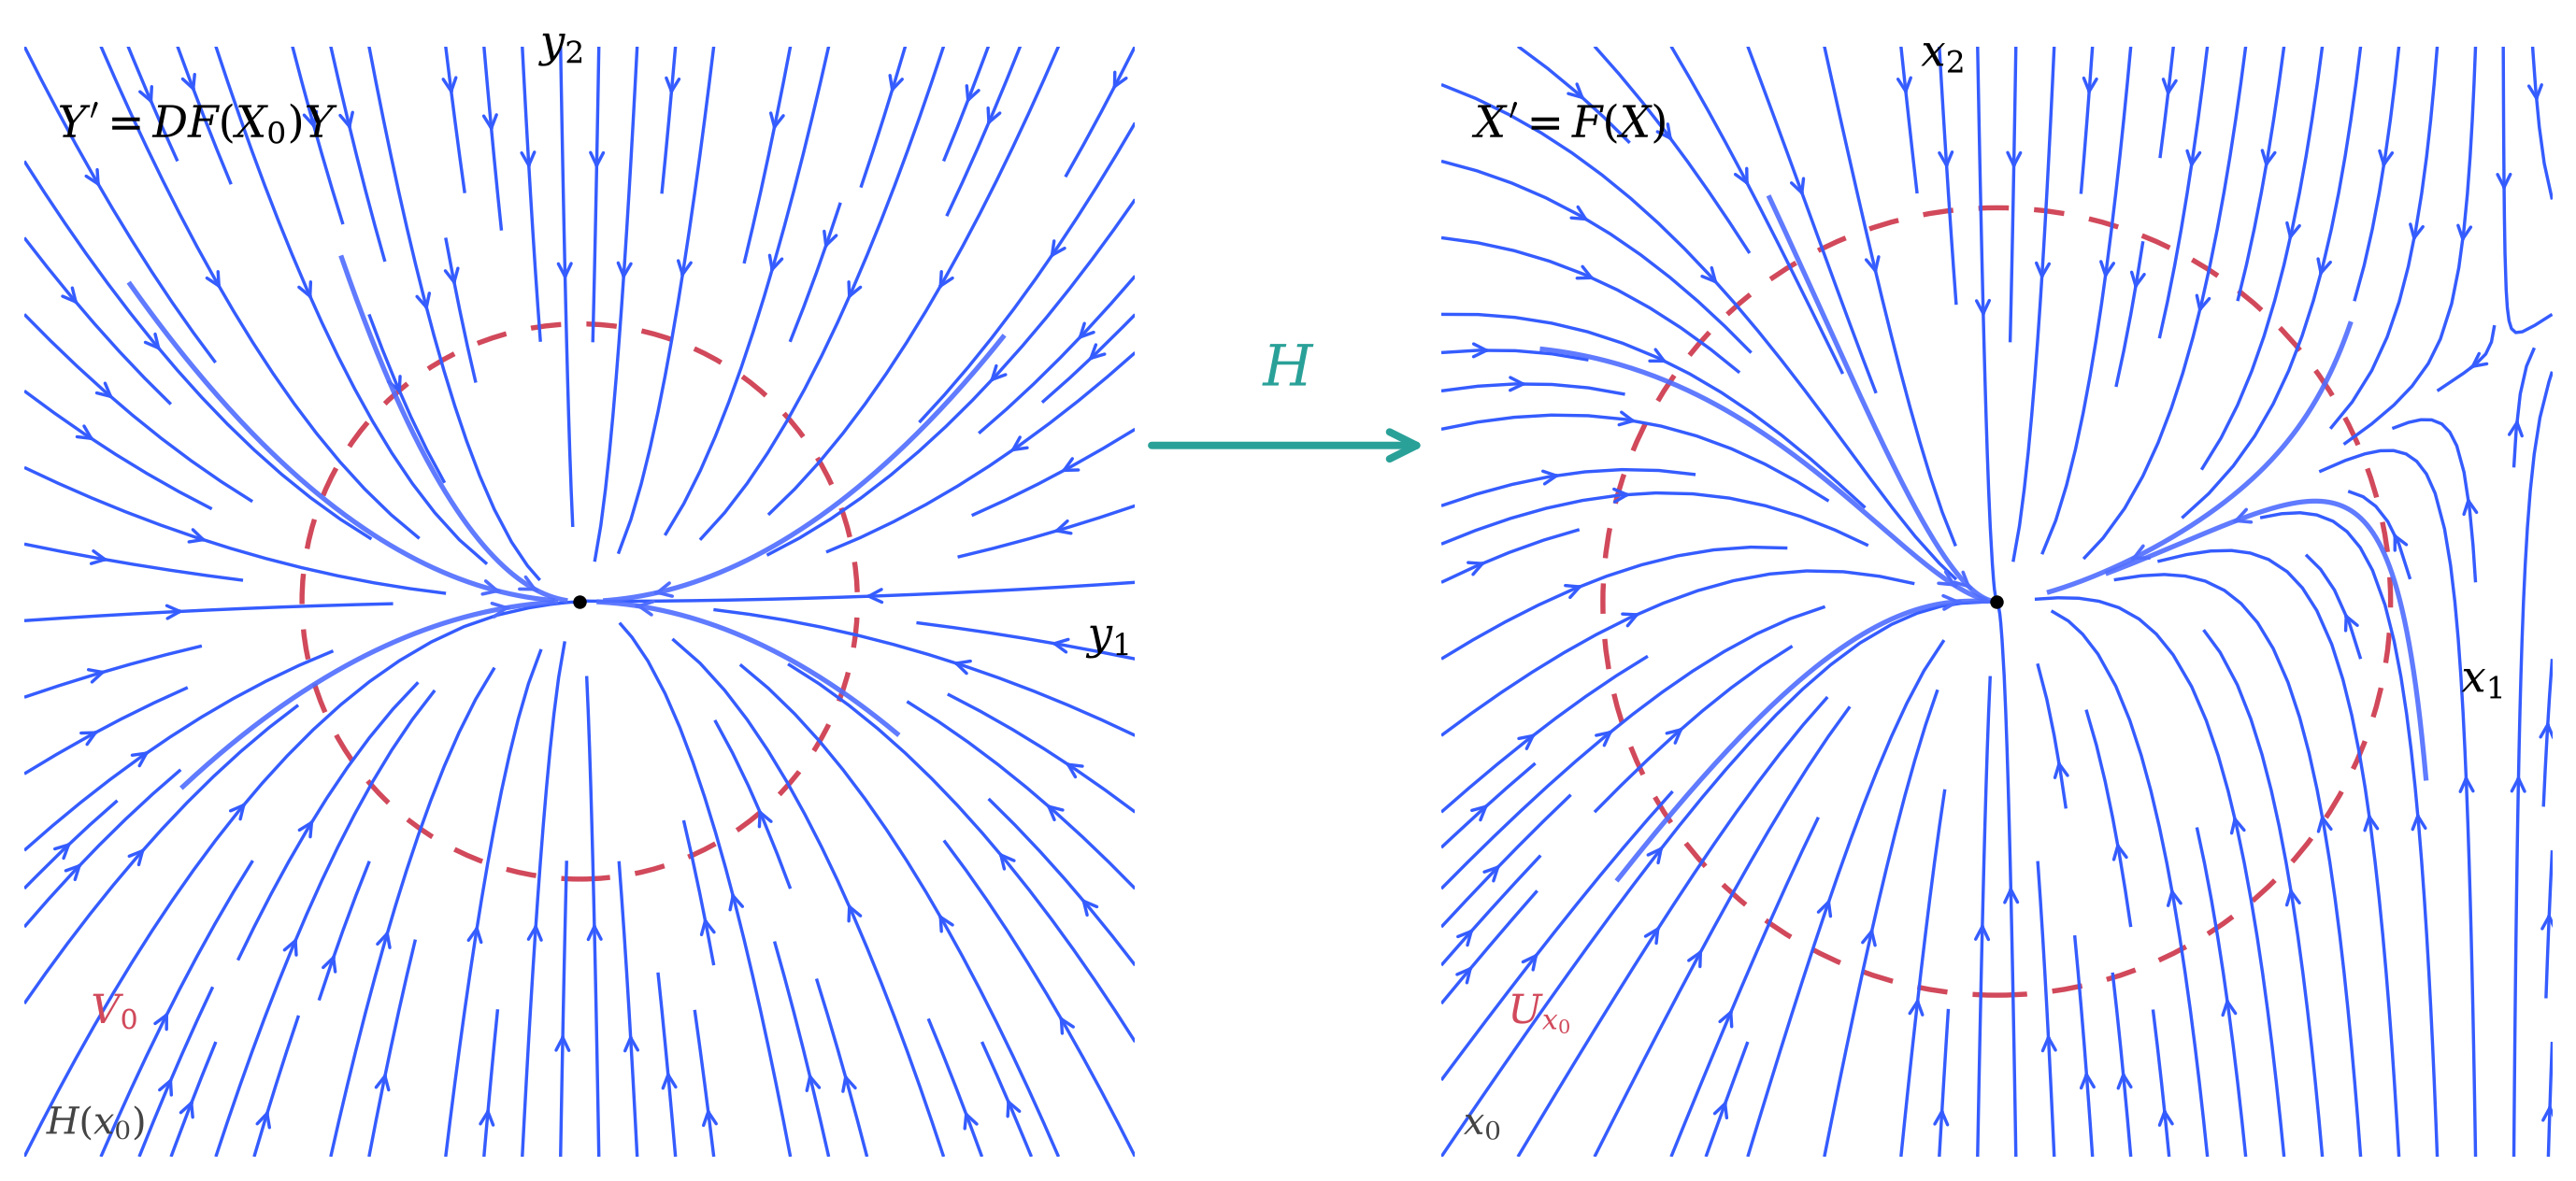
\includegraphics[width=0.98\linewidth]{fig_17_hg_conjugacion_local.png}
\caption{Retratos de fase locales alrededor de \(X_0=(0,0)\): a la izquierda el sistema linealizado \(Y'=DF(X_0)Y\), a la derecha el sistema no lineal \(X'=F(X)\), unidos por la conjugaci\'on local \(H\).}
\end{figure}

\medskip

\textbf{Ejemplo}

\[
x_1'=-x_1+x_1^2
\]

\[
x_2'=-2x_2+x_1^2
\]

\textbf{Puntos de equilibrio}

\[
x_1'=-x_1+x_1^2=0 \iff x_1=0 \ \text{o}\ x_1=1
\]

\[
-2x_2=x_1^2
\]

\[
\begin{array}{rcl}
\text{i)} & x_1=0 &\Rightarrow x_2=0 \\
          &       &\Rightarrow X_0=(0,0),\ \text{punto de equilibrio}
\end{array}
\]

\[
\begin{array}{rcl}
\text{ii)} & x_1=1 &\Rightarrow 2x_2=1 \Rightarrow x_2=\dfrac12 \\
           &       &\Rightarrow X_1=\left(1,\dfrac12\right),\ \text{punto de equilibrio}
\end{array}
\]

\[
\text{¿Cuál es el comportamiento del flujo cerca de los puntos de equilibrio?}
\]

\[
\text{Observemos que:}\qquad
J(X)=DF(X)=
\begin{pmatrix}
2x_1-1 & 0\\
2x_1 & -2
\end{pmatrix}
\]

\[
\text{i) }X_0=(0,0):\qquad
A=J(X_0)=
\begin{pmatrix}
-1 & 0\\
0 & -2
\end{pmatrix},
\qquad Y'=DF(X_0)Y
\]

\[
Y_1'=-Y_1,\qquad Y_2'=-2Y_2
\]

\[
p(\lambda)=\det(A-\lambda I)
=
\det\begin{pmatrix}
-1-\lambda & 0\\
0 & -2-\lambda
\end{pmatrix}
= (\lambda+1)(\lambda+2)
\]

\[
\lambda_1=-1,\qquad \lambda_2=-2
\ \text{valores propios}
\]

\[
DF(X_0)\ \text{no tiene valores propios nulos ni con parte real nula}
\]

\[
\Rightarrow X_0\ \text{es hiperb\'olico}
\]

\newpage

\textbf{Flujo y conjugacion}

\[
y' = ay, \qquad y(t)=e^{at}y_0, \qquad y_0=y(0)
\]

\[
\text{Ansatz} \leftrightarrow y(t)=e^{\lambda t}v \text{ en el s.e. } x'=Ax
\]

\[
\lambda,\ v \text{ son valores propios y vectores propios de } A
\]

\[
\lambda_1>0,\qquad \lambda_2<0
\]

\[
y_1(t)=e^{\lambda_1 t}v_1,\qquad y_2(t)=e^{\lambda_2 t}v_2
\]

\[
y(t)=c_1e^{\lambda_1 t}v_1+c_2e^{\lambda_2 t}v_2
\]

\medskip

\textbf{Vector propio \(V_1\), \(\lambda_1=-1\)}

\[
AV_1=\lambda_1 V_1
\]

\[
\Leftrightarrow AV_1-\lambda_1 I V_1=\vec{0}
\]

\[
\Rightarrow (A-\lambda_1 I)V_1=\vec{0}.
\]

\[
A-\lambda_1 I=
\begin{pmatrix}
-1 & 0\\
0 & -2
\end{pmatrix} +
\begin{pmatrix}
1 & 0\\
0 & 1
\end{pmatrix}
=
\begin{pmatrix}
0 & 0\\
0 & -1
\end{pmatrix}
\]

\[
(A-\lambda_1 I)V_1=\vec{0}
\Leftrightarrow
\begin{pmatrix}
0 & 0\\
0 & -1
\end{pmatrix}
\binom{v_1}{v_2}
=
\binom{0}{0}
\]

\[
\Rightarrow -v_2=0
\]

\[
\Rightarrow v_2=0
\]

\[
V_1=\binom{1}{0}
\]

\[
Y_1(t)=e^{\lambda_1 t}V_1=e^{-t}\binom{1}{0}
\]

\[
\lambda_2=-2
\]

\[
A-\lambda_2 I=
\begin{pmatrix}
-1 & 0\\
0 & -2
\end{pmatrix}
-
\begin{pmatrix}
-2 & 0\\
0 & -2
\end{pmatrix}
=
\begin{pmatrix}
1 & 0\\
0 & 0
\end{pmatrix}
\]

\[
\vec{0}=(A-\lambda_2 I)V_2
\Leftrightarrow
\binom{0}{0}
=
\begin{pmatrix}
1 & 0\\
0 & 0
\end{pmatrix}
\binom{w_1}{w_2}
\]

\[
w_1=0
\]

\[
\text{tomamos }w_2=1
\]

\[
V_2=\binom{0}{1}
\]

\[
Y_2(t)=e^{\lambda_2 t}V_2=e^{-2t}\binom{0}{1}
\]

\begin{figure}[H]
\centering
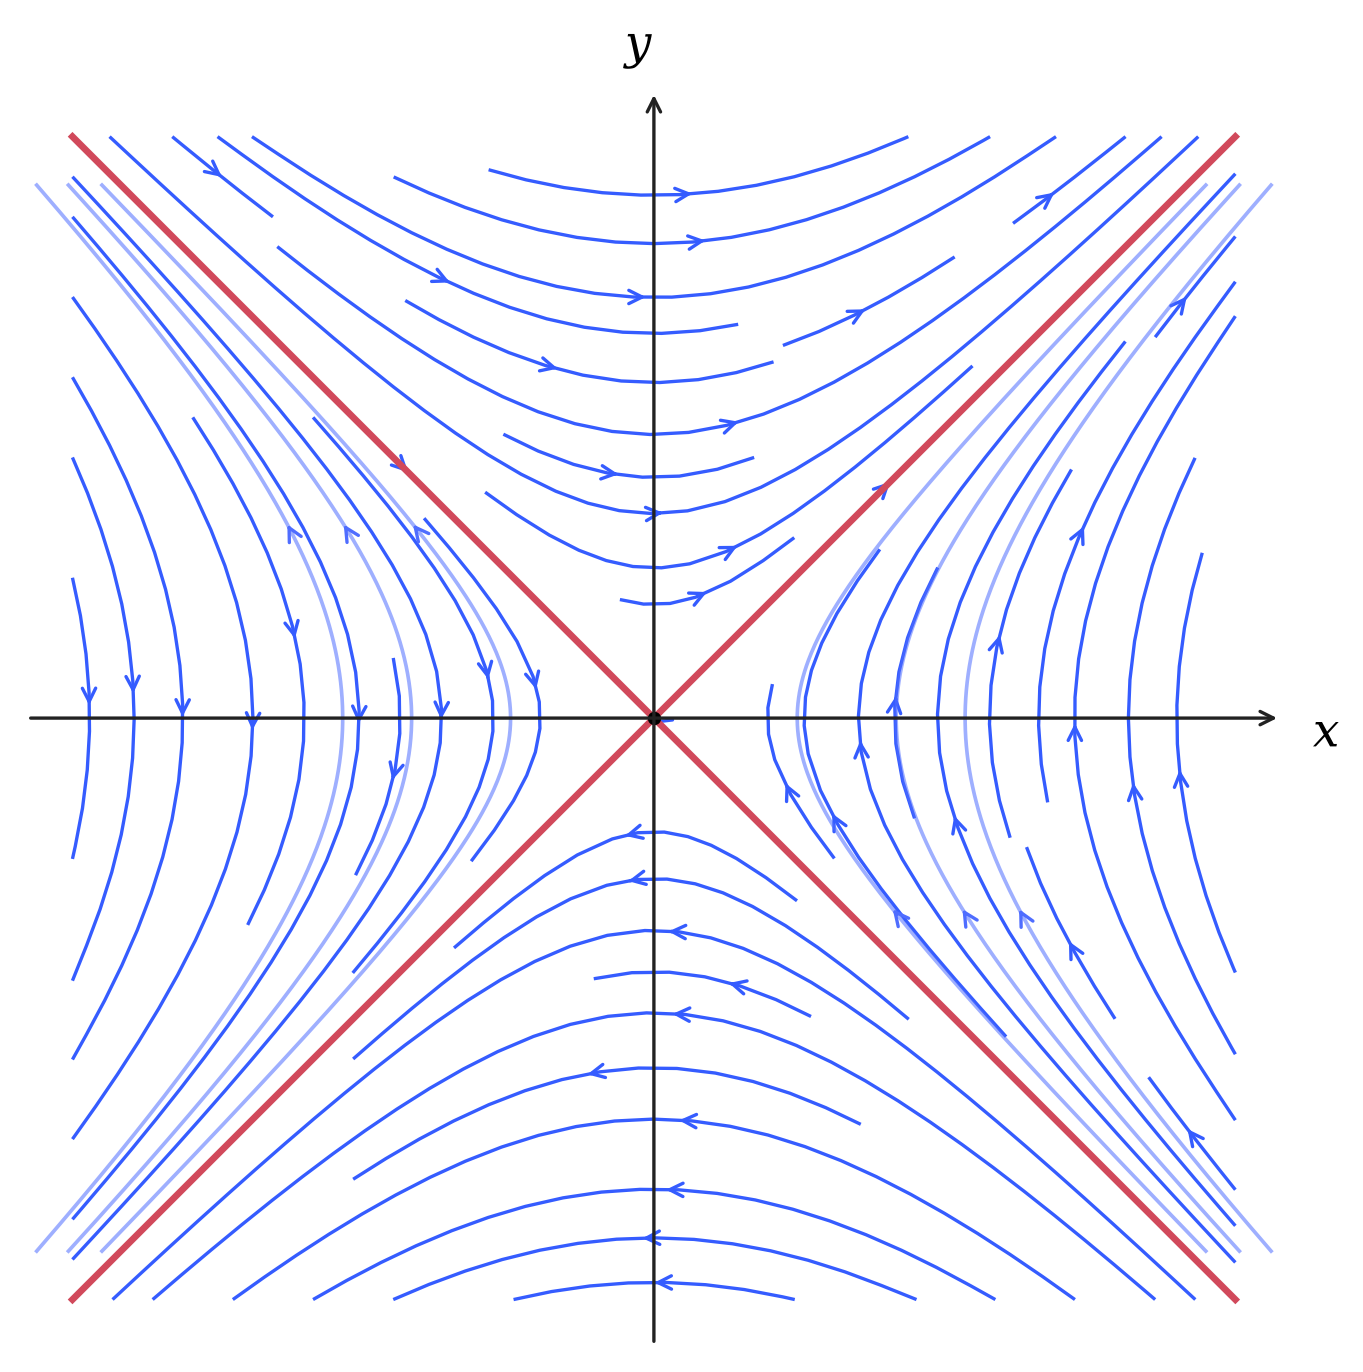
\includegraphics[width=0.94\linewidth]{fig_14_flujo_silla.png}
\caption{Retrato de fase tipo silla con separatrices y trayectorias esquematicas.}
\end{figure}

\[
\text{Sea } x'=f(x), \text{ en } \mathbb{R}^n \text{ de clase } C^1
\]

\[
\text{se tiene el llamado flujo asociado } \varphi(t)
\]

\[
\varphi:\mathbb{R}\times\mathbb{R}^n\to\mathbb{R}^n,\qquad (t,x)\mapsto \varphi(t,x)=\varphi_t(x)
\]

\[
\text{El cual satisface las propiedades}
\]

\[
\varphi(0,x)=\varphi_0(x)=x
\]

\[
\varphi(s,\varphi(t,x))=\varphi_{s+t}(x)
\]

\[
\frac{d}{dt}\varphi_t(x)=F(\varphi_t(x))
\]

\[
\varphi_t(x)=x(t)=xe^{at}, \qquad \varphi_0(x)=x(0)=x
\]

\[
\varphi_s(\varphi_t(x))=\varphi_s(xe^{at})=xe^{a(s+t)}=\varphi_{s+t}(x)
\]

\begin{figure}[H]
\centering
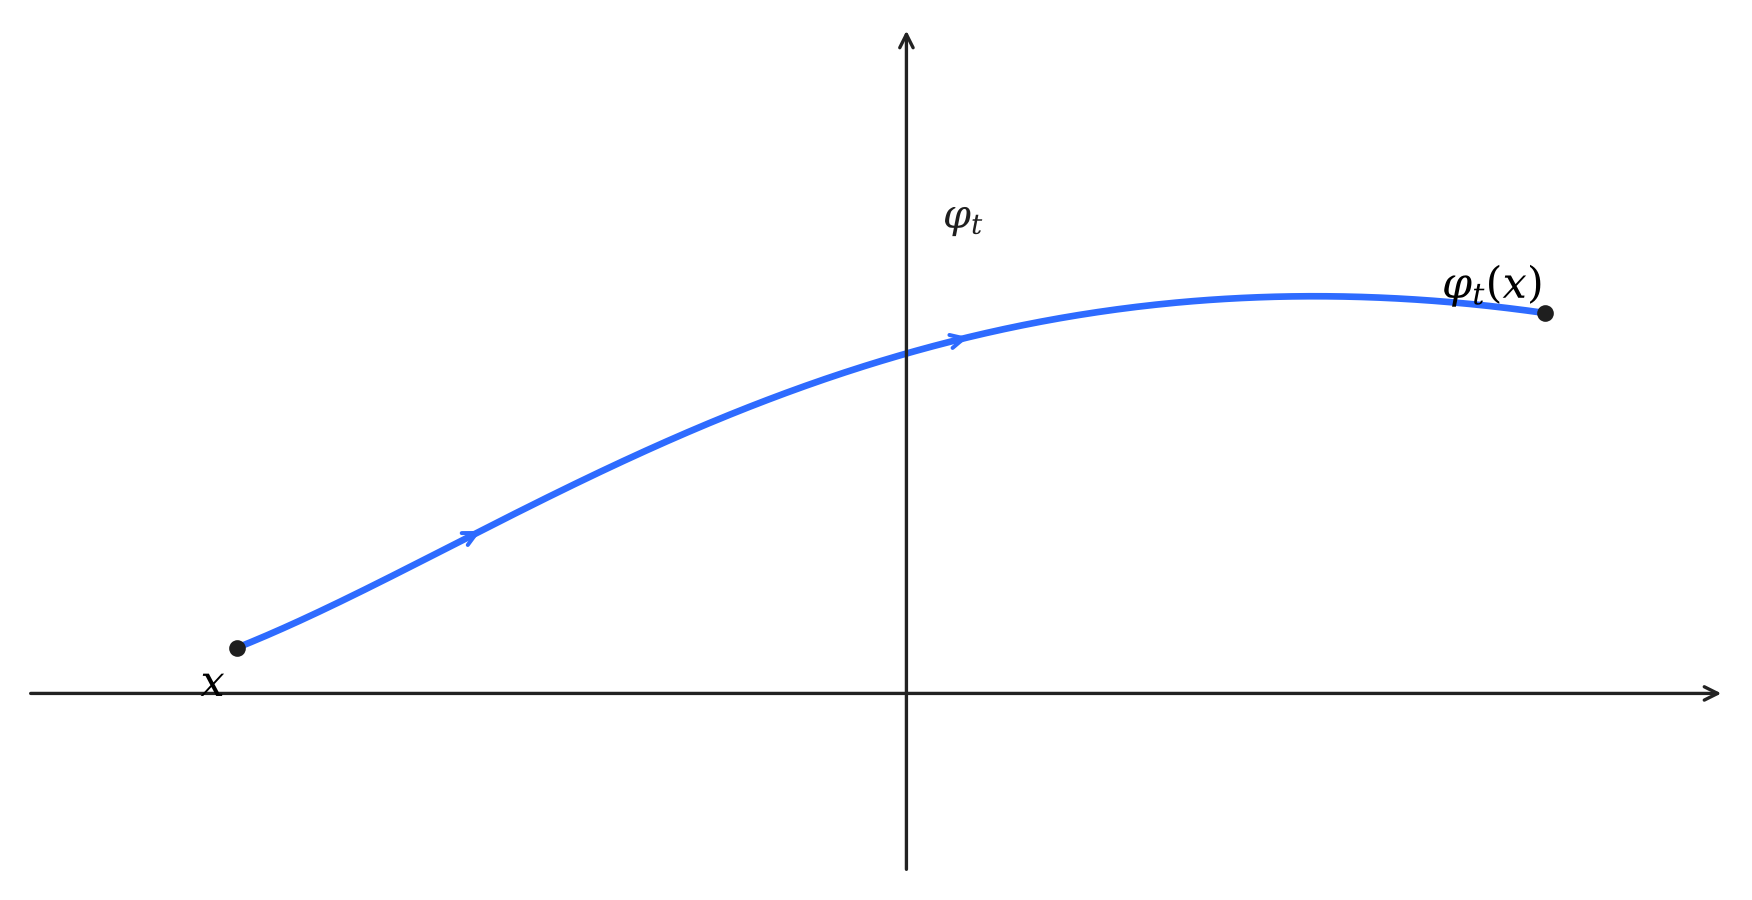
\includegraphics[width=0.96\linewidth]{fig_15_flujo_orbita.png}
\caption{Trayectoria de una solucion bajo el flujo \(\varphi_t\).}
\end{figure}

\begin{figure}[H]
\centering
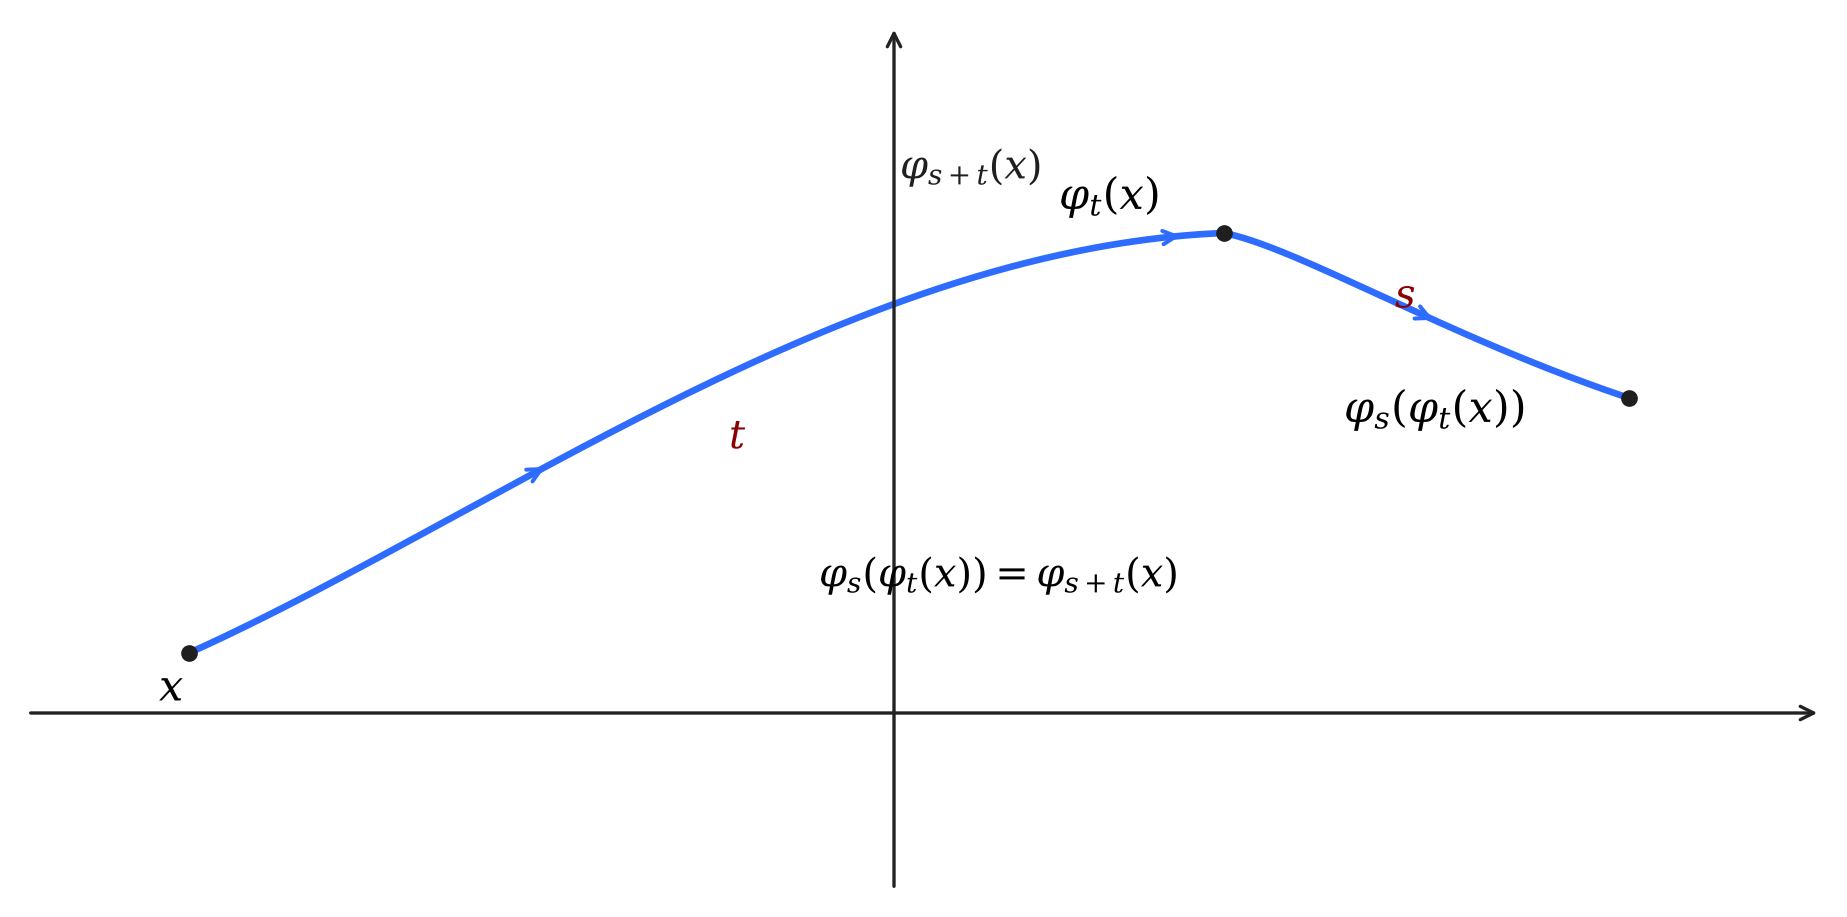
\includegraphics[width=0.96\linewidth]{fig_16_flujo_composicion.png}
\caption{Ilustracion de la propiedad de composicion \(\varphi_s(\varphi_t(x))=\varphi_{s+t}(x)\).}
\end{figure}

\[
\text{Sean } x'=F(x), \qquad y'=G(y) \text{ de clase } C^1
\]

\[
x_0,\ y_0 \text{ puntos de equilibrio de (a) y (b) respectivamente}
\]

\[
\varphi_t(x),\ \psi_t(y) \text{ son sus flujos correspondientes}
\]

\[
\text{Decimos que (a) y (b) son localmente topologicamente conjugados alrededor de }x_0\text{ y }y_0\text{ si}
\]

\[
\exists\ \text{vecindades }U_{x_0}, V_{y_0}
\]

\[
\exists\ H:U_{x_0}\to V_{y_0}\ \text{un homeomorfismo}
\]

\[
H(\varphi_t(x))=\psi_t(H(x))
\]

\medskip

\textbf{Soluci\'on de la tarea}

\[
J(X)=
\begin{pmatrix}
2x_1-1 & 0\\
2x_1 & -2
\end{pmatrix}
\qquad\Rightarrow\qquad
J(X_1)=
\begin{pmatrix}
1 & 0\\
2 & -2
\end{pmatrix}
\]

\[
p(\lambda)=\det(J(X_1)-\lambda I)
=
\det\begin{pmatrix}
1-\lambda & 0\\
2 & -2-\lambda
\end{pmatrix}
=(1-\lambda)(-2-\lambda)
\]

\[
\lambda_1=1,\qquad \lambda_2=-2
\]

\[
\Rightarrow X_1=\left(1,\dfrac12\right)\ \text{es hiperb\'olico y de tipo silla}
\]

\[
\text{En variables locales }Y=X-X_1,\ \text{el sistema linealizado es }Y'=J(X_1)Y
\]

\[
Y(t)=c_1e^{t}\binom{3}{2}+c_2e^{-2t}\binom{0}{1}
\]

\[
\varphi_t(Y_0)=
\left(
e^t Y_{0,1},
\dfrac{2}{3}(e^t-e^{-2t})Y_{0,1}+e^{-2t}Y_{0,2}
\right)
\]

\noindent Por Hartman-Grobman, el sistema no lineal cerca de \(X_1\) es topol\'ogicamente conjugado a esta silla lineal.

\noindent Las soluciones se acercan a \(X_1\) sobre la variedad estable y se alejan por la variedad inestable.

\newpage

\textbf{No-ejemplo}

\begin{figure}[H]
\centering
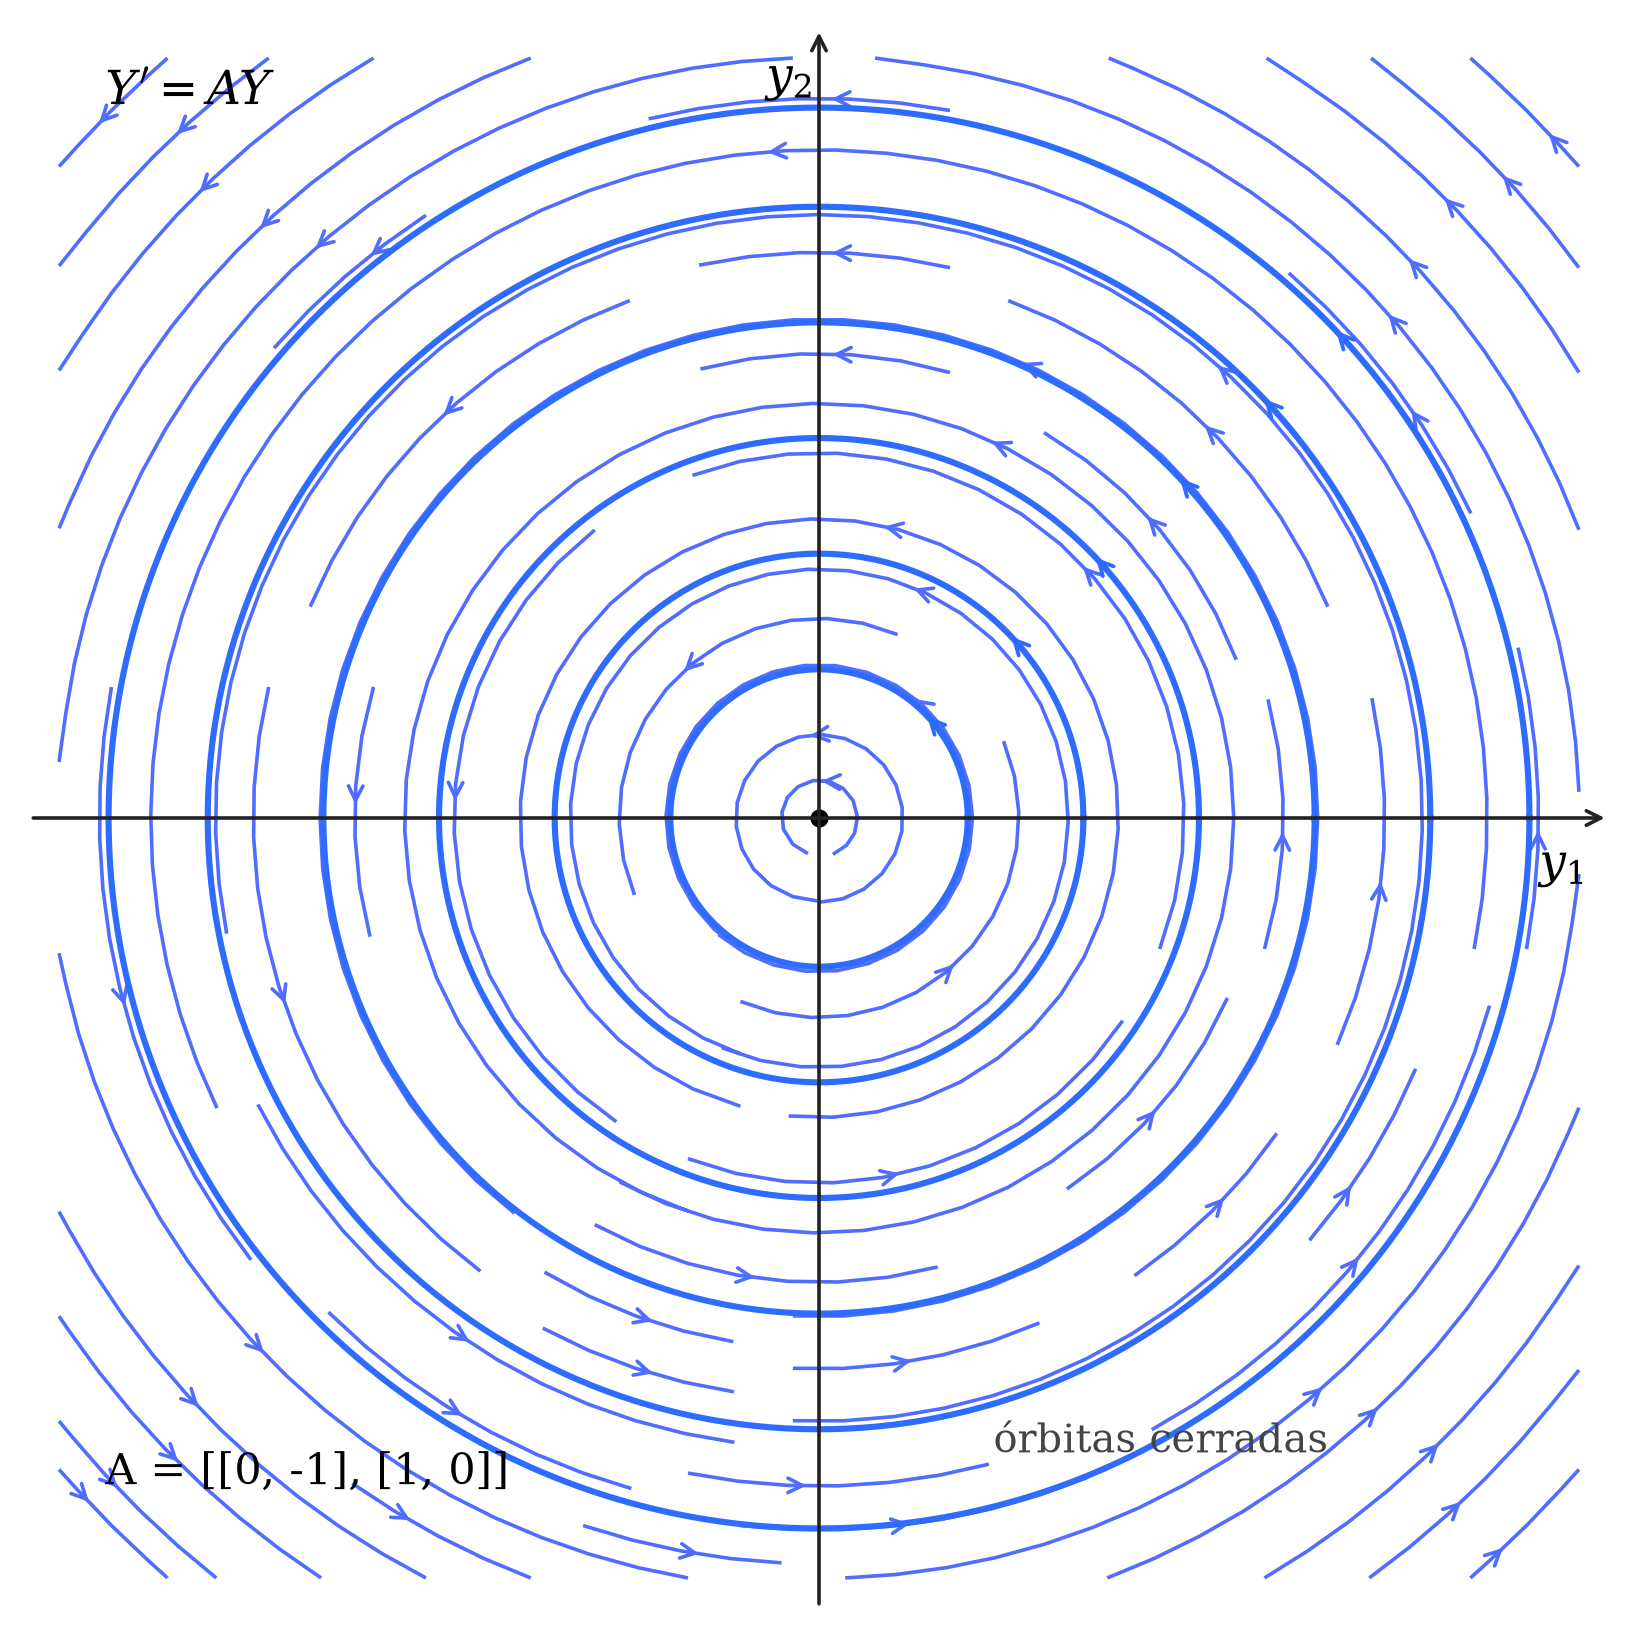
\includegraphics[width=0.94\linewidth]{fig_18_sistema_lineal_periodico.png}
\caption{Retrato de fase del sistema linealizado \(Y'=AY\), con \(A=\begin{pmatrix}0 & -1\\ 1 & 0\end{pmatrix}\): centro en el origen y trayectorias cerradas, por lo que las soluciones son peri\'odicas.}
\end{figure}

\begin{figure}[H]
\centering
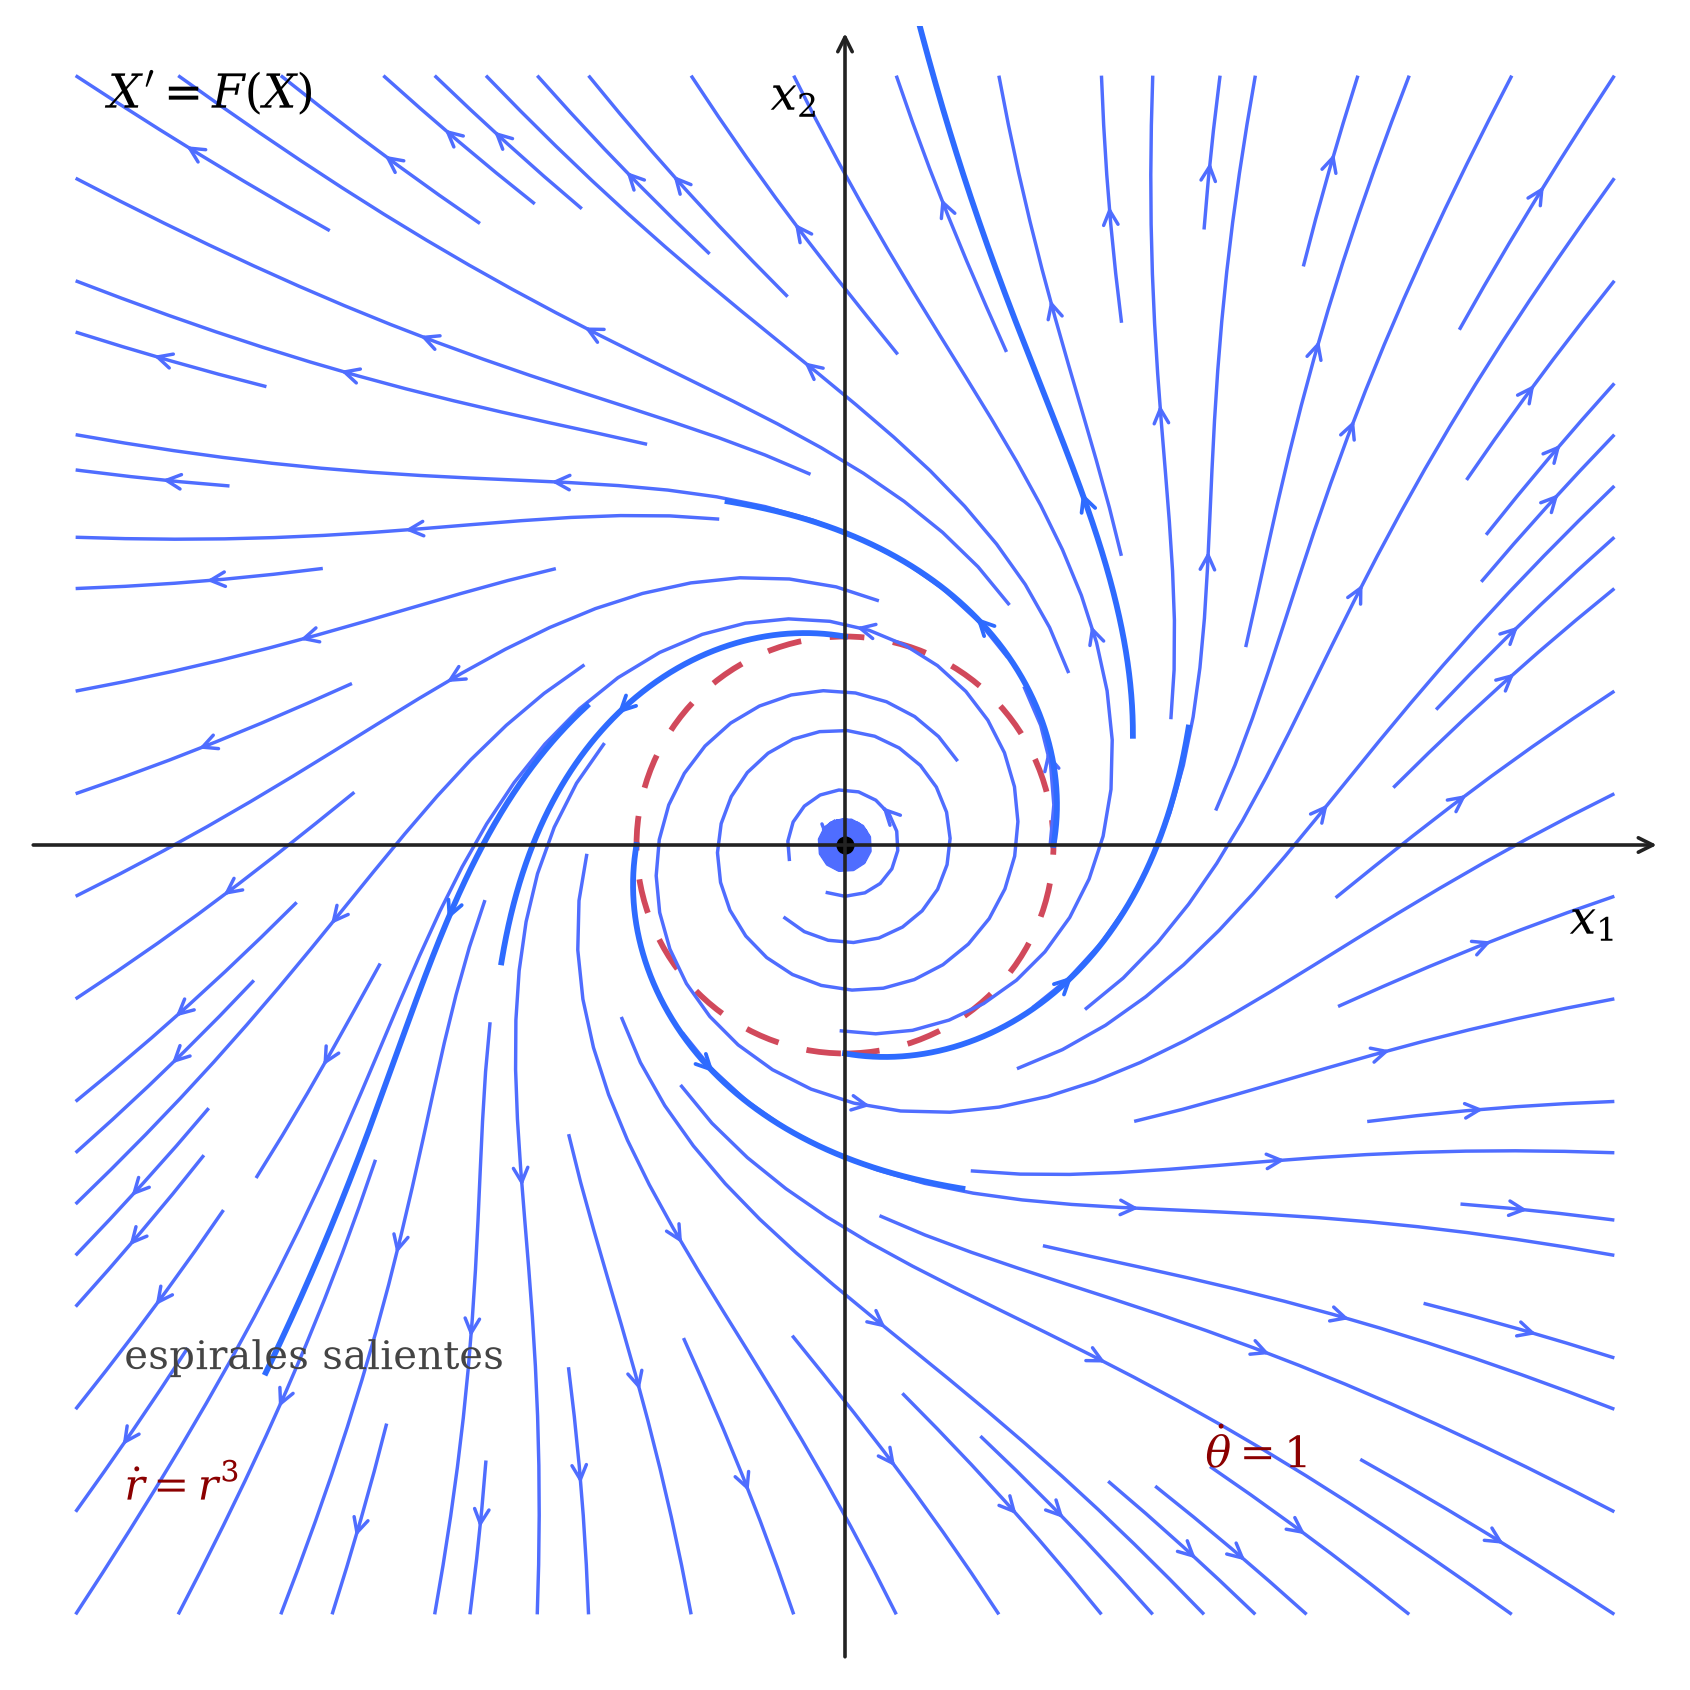
\includegraphics[width=0.94\linewidth]{fig_19_no_ejemplo_espiral.png}
\caption{Retrato de fase del no-ejemplo no lineal cerca del origen: las trayectorias son espirales salientes, coherentes con \(\dot r=r^3\) y \(\dot\theta=1\).}
\end{figure}

\textbf{Sistema no lineal}

\[
x'=-y+x(x^2+y^2)=-y+x^3+xy^2
\]

\[
y'=x+y(x^2+y^2)=x+x^2y+y^3
\]

\textbf{Ejercicio:} el origen, punto de equilibrio. ¿Es único?

\[
(0,0)=X_0\ \text{no es hiperb\'olico}
\]

\[
DF(X)=
\begin{pmatrix}
3x^2+y^2 & -1+2xy\\
1+2xy & x^2+3y^2
\end{pmatrix}
\]

\[
DF(X_0)=
\begin{pmatrix}
0 & -1\\
1 & 0
\end{pmatrix}
\]

\textbf{En \(Y\)'s:}

\[
(A)\quad
\begin{cases}
y_1'=-y_2,\\
y_2'=y_1,
\end{cases}
\qquad
Y'=
\begin{pmatrix}
0 & -1\\
1 & 0
\end{pmatrix}
Y
\]

\[
p(\lambda)=\det(A-\lambda I)
=
\det\begin{pmatrix}
-\lambda & -1\\
1 & -\lambda
\end{pmatrix}
=\lambda^2+1=0
\]

\[
\Rightarrow \lambda=\pm i
\]

\textbf{Respuesta de la tarea}

\[
Y(t)=r_0\binom{\cos(t+\theta_0)}{\sin(t+\theta_0)}
\]

\[
\dot r=0,\qquad \dot\theta=1
\]

\[
\Rightarrow \text{las soluciones son circunferencias y, por tanto, peri\'odicas de periodo }2\pi
\]

\textbf{Cambio a coordenadas polares en el no-ejemplo}

\[
r^2=x^2+y^2,\qquad x=r\cos\theta,\qquad y=r\sin\theta
\]

\[
2r\dot r=2x\dot x+2y\dot y
\]

\[
\Rightarrow \dot r=\frac{x\dot x+y\dot y}{r}
\]

\[
=\frac{x[-y+x(x^2+y^2)]+y[x+y(x^2+y^2)]}{r}
\]

\[
=\frac{-xy+x^2(x^2+y^2)+xy+y^2(x^2+y^2)}{r}
\]

\[
=\frac{(x^2+y^2)(x^2+y^2)}{r}
=\frac{r^4}{r}=r^3
\]

\[
\dot\theta=\frac{x\dot y-y\dot x}{x^2+y^2}
\]

\[
=\frac{x[x+y(x^2+y^2)]-y[-y+x(x^2+y^2)]}{x^2+y^2}=1
\]

\[
\therefore \dot r=r^3,\qquad \dot\theta=1
\]

\noindent Las trayectorias del no-ejemplo son espirales salientes y el origen no es hiperb\'olico.

\newpage
\textbf{Isoclinas (nulas)}

\begin{figure}[H]
\centering
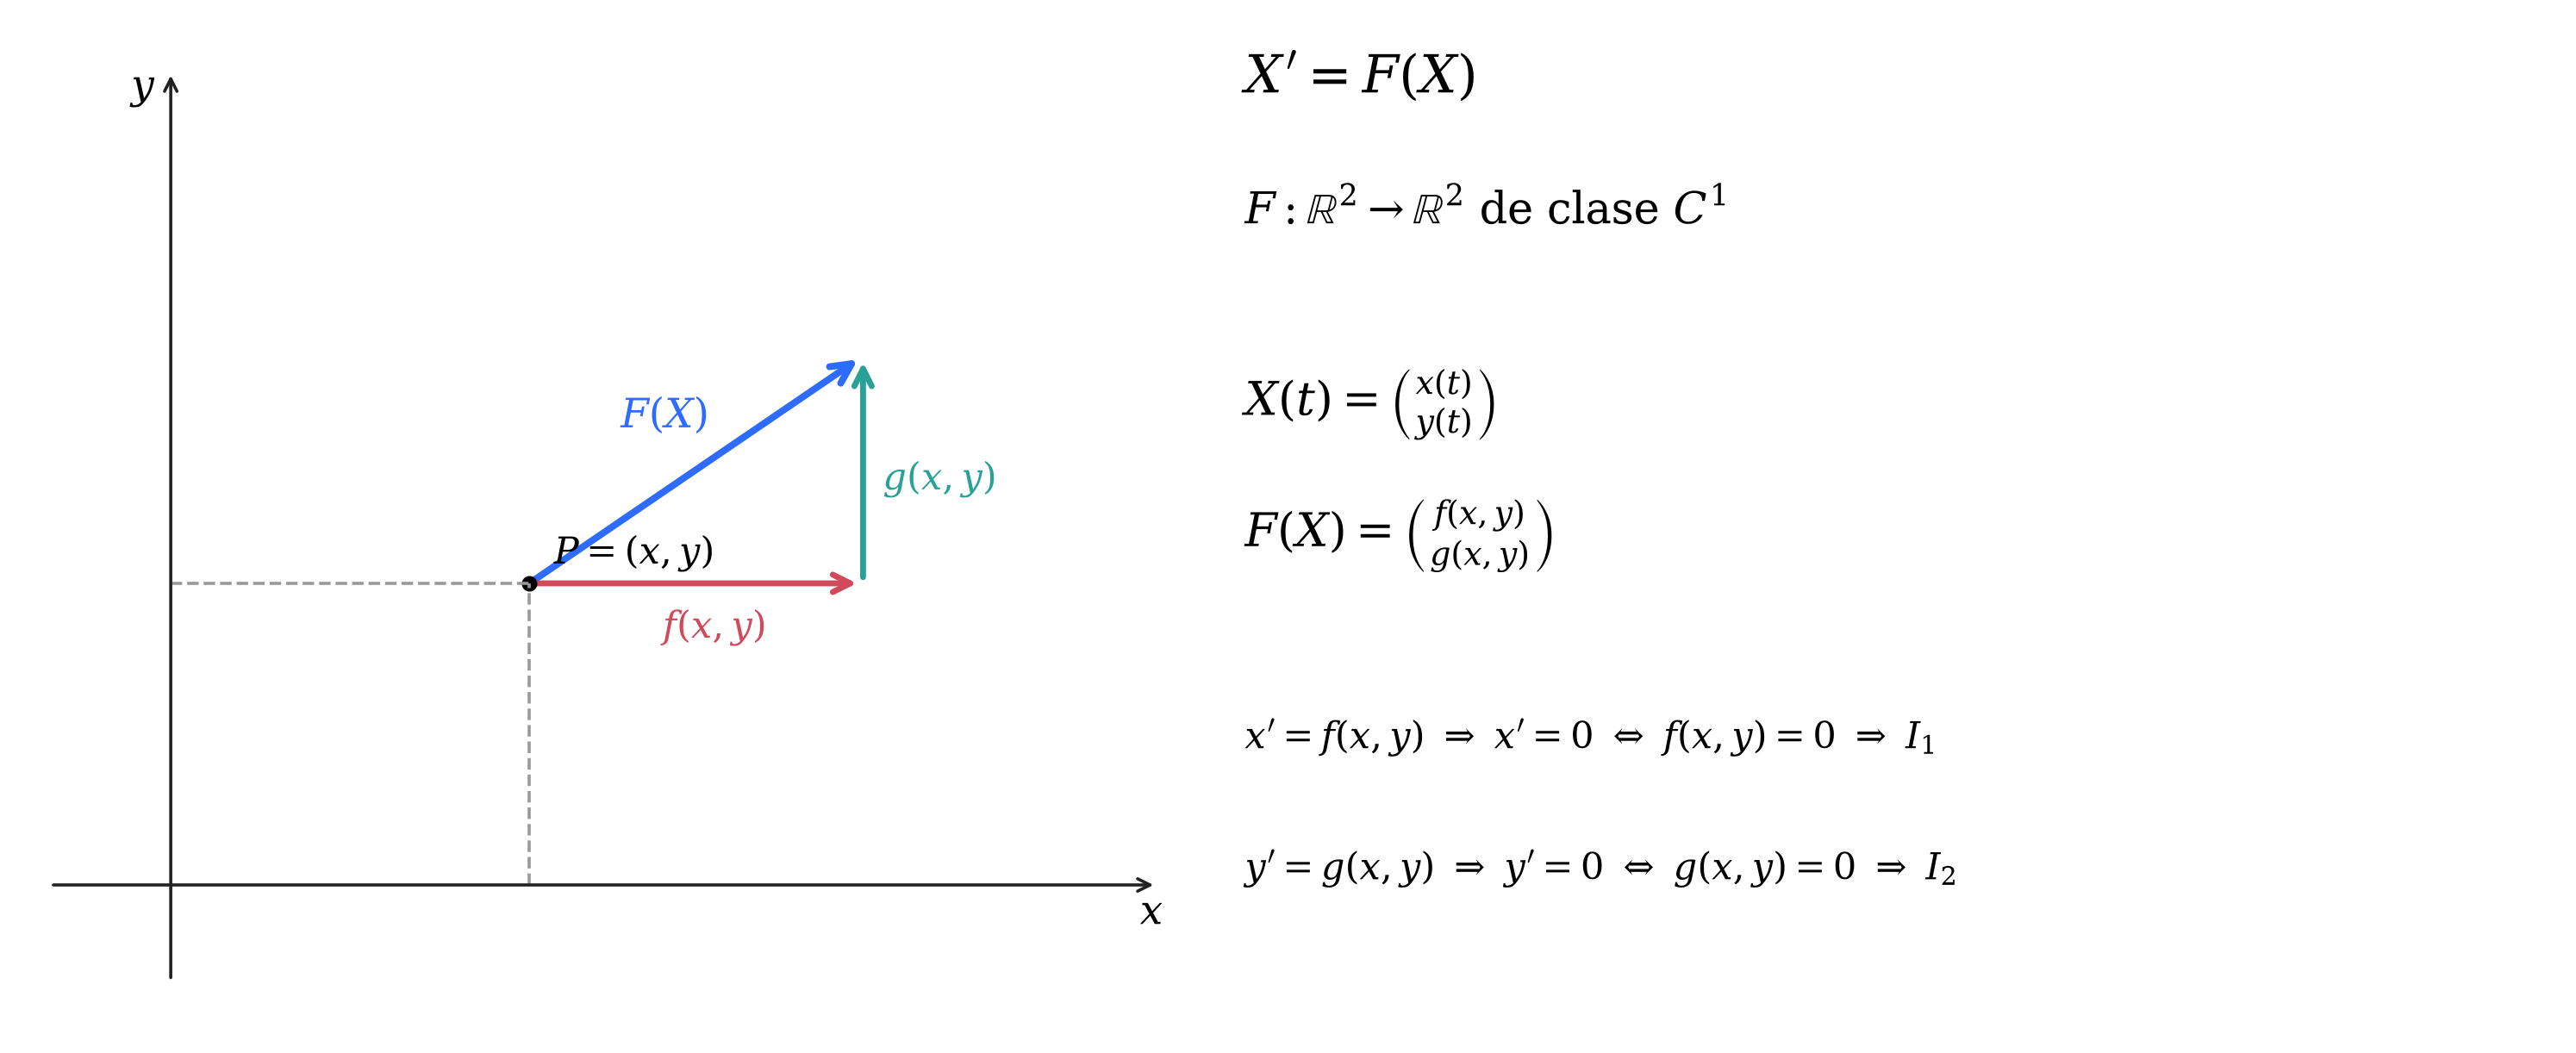
\includegraphics[width=0.92\linewidth]{fig_20_isoclinas_esquema.png}
\end{figure}

\begin{figure}[H]
\centering
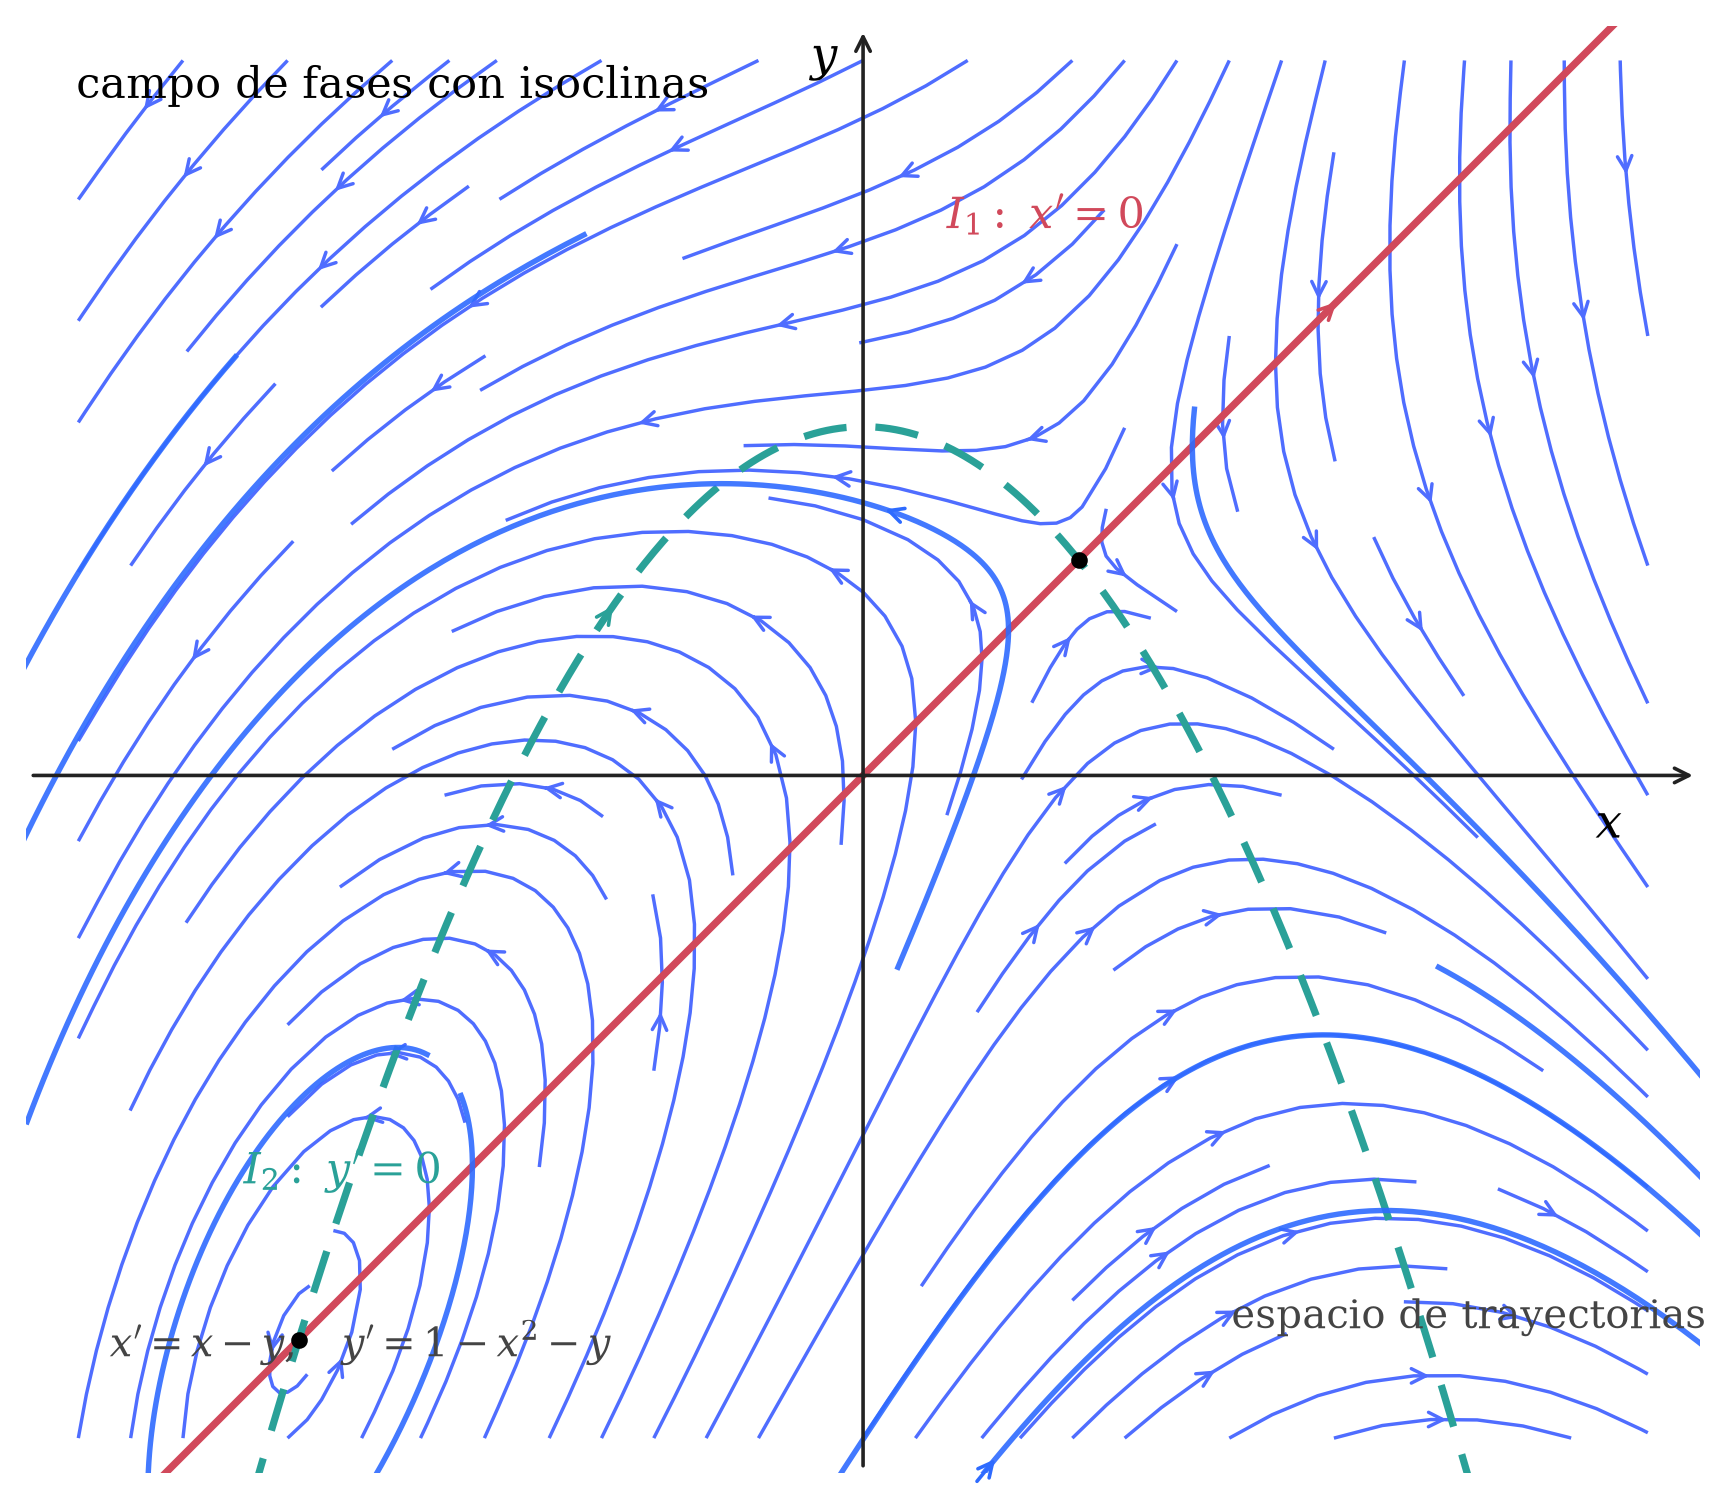
\includegraphics[width=0.92\linewidth]{fig_21_isoclinas_retrato.png}
\end{figure}

\begin{figure}[H]
\centering
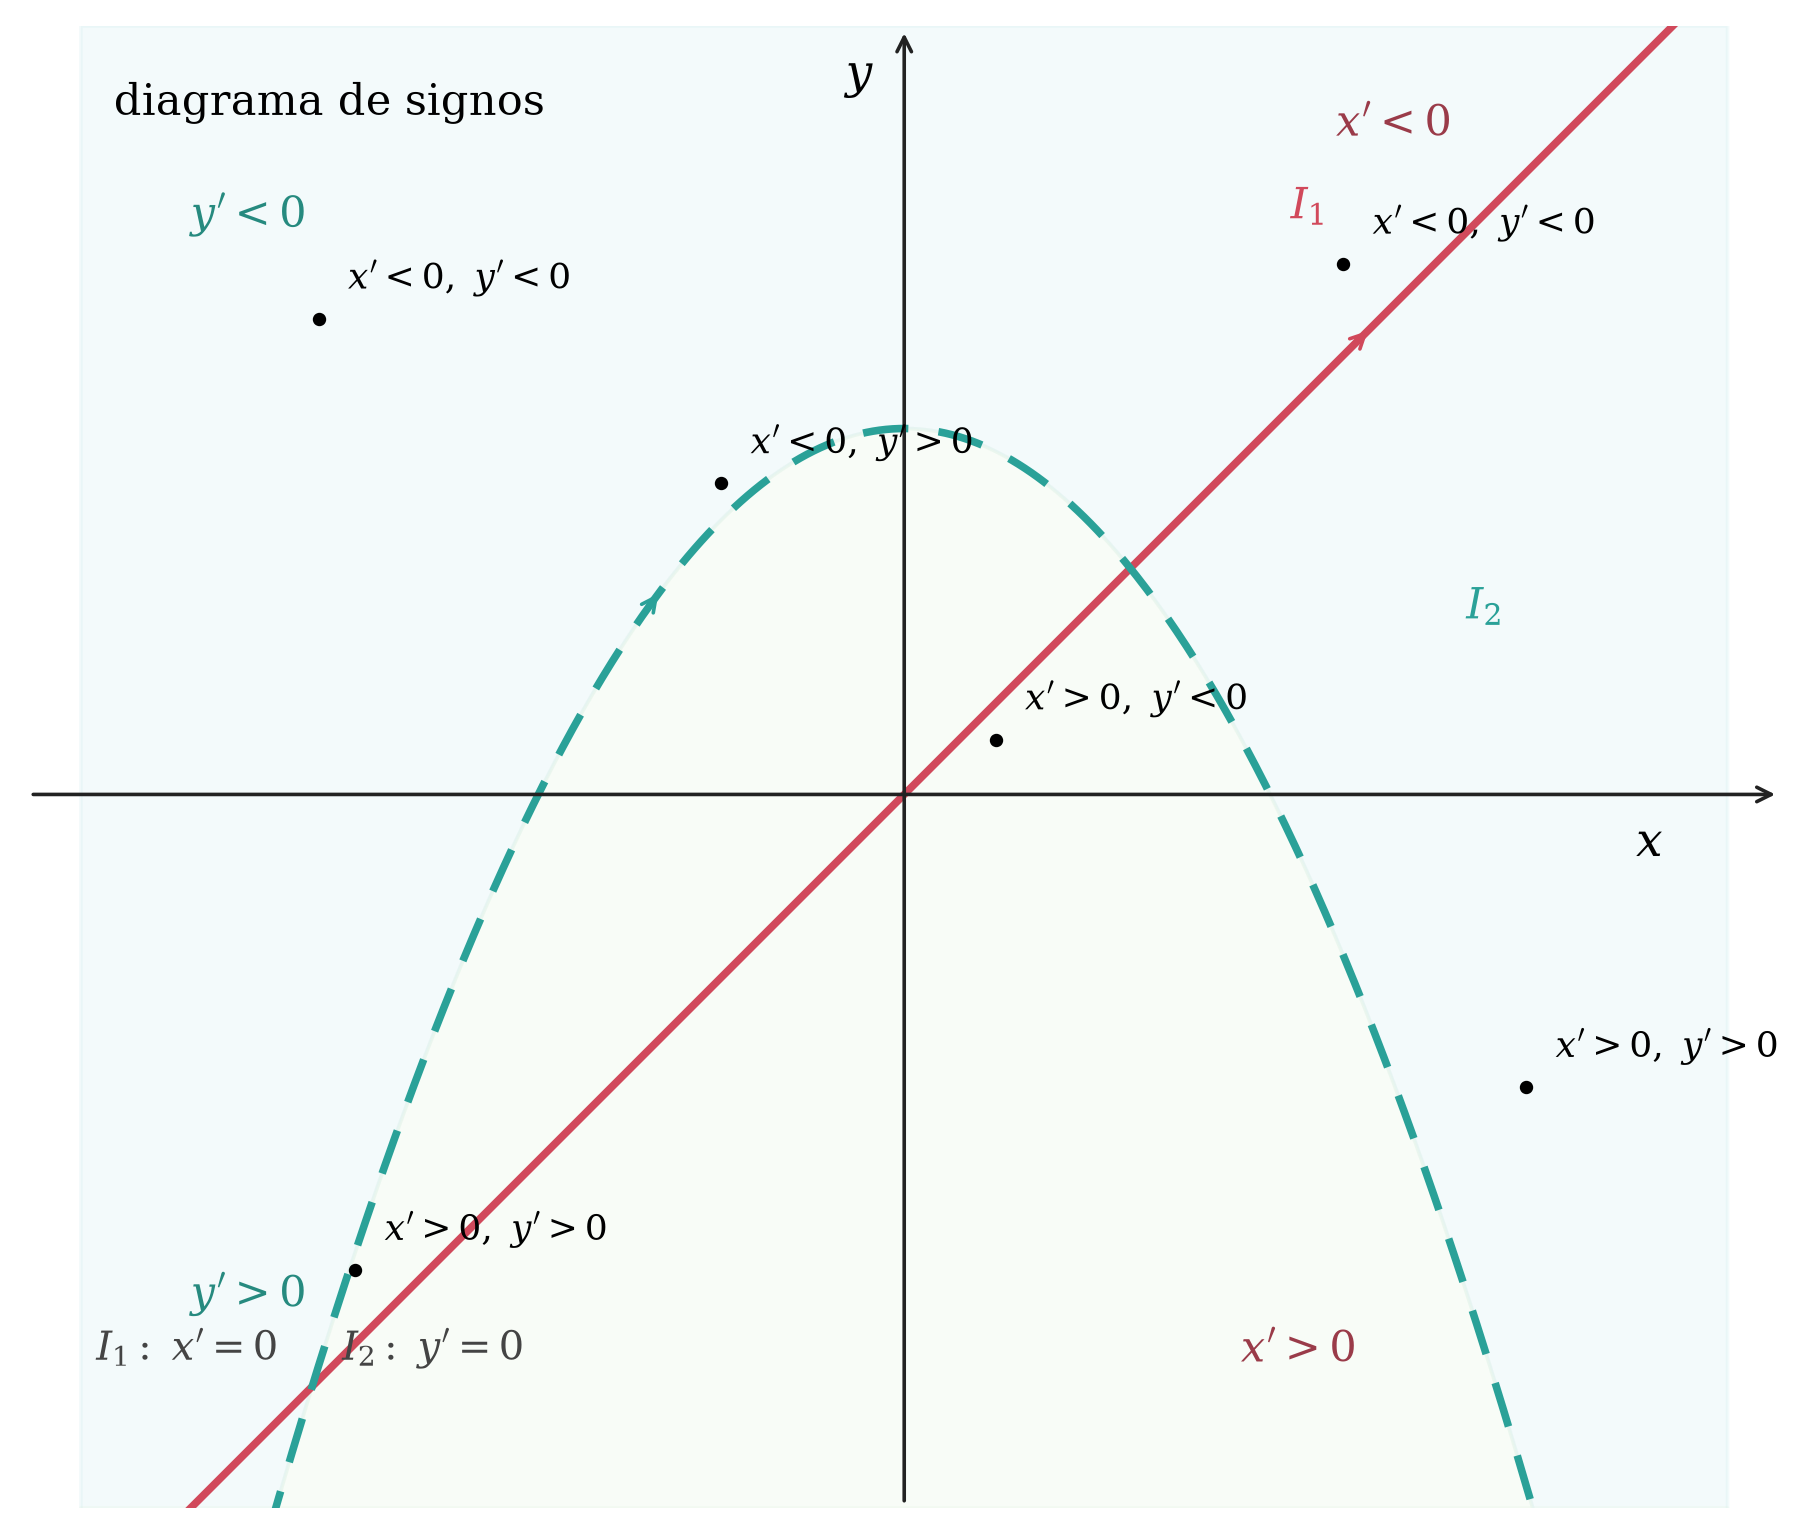
\includegraphics[width=0.92\linewidth]{fig_22_isoclinas_signos.png}
\end{figure}

\[
X' = F(X), \qquad F:\mathbb{R}^2 \to \mathbb{R}^2 \text{ de clase } C^1
\]

\[
X(t)=\binom{x(t)}{y(t)}, \qquad F(X)=\binom{f(x,y)}{g(x,y)}
\]

\[
x'=f(x,y)\ \Rightarrow\ x'=0\ \Leftrightarrow\ f(x,y)=0\ \Rightarrow\ I_1
\]

\[
y'=g(x,y)\ \Rightarrow\ y'=0\ \Leftrightarrow\ g(x,y)=0\ \Rightarrow\ I_2
\]

\noindent En \(I_1\), \(F=\binom{0}{g(x,y)}\).

\noindent En \(I_2\), \(F=\binom{f(x,y)}{0}\).

\noindent Las isoclinas \(I_1\) e \(I_2\) dividen el plano en regiones donde se lee el signo de cada componente del campo.

\noindent \naglecite{cap.~5: esta partici\'on del plano fase es el punto de partida del an\'alisis cualitativo.}

\newpage
\textbf{Isoclinas nulas y an\'alisis de signos}

\[
x' = x(1-x-y)=x-xy-x^2
\]

\[
y' = y(1-x)=y-xy
\]

\noindent Para describir la din\'amica global, conviene proceder en dos etapas:

\begin{enumerate}
\item Puntos de equilibrio y estabilidad local.
\item Isoclinas nulas y signos de \(x'\) y \(y'\).
\end{enumerate}

\noindent \textbf{ii) Isoclinas nulas:}

\noindent \textbf{Para \(x'\):}

\[
x(1-x-y)=0
\iff x=0\ \text{o}\ 1-x-y=0
\iff x=0\ \text{o}\ y=1-x
\]

\noindent \textbf{Para \(y'\):}

\[
y(1-x)=0
\iff y=0\ \text{o}\ x=1
\]

\noindent Los ejes coordenados positivos son invariantes.

\noindent Estas isoclinas nulas dividen el plano en regiones donde se leen los signos de \(x'\) y \(y'\).

\noindent La forma general del modelo de competencia puede escribirse como

\[
x'=\alpha x-\beta xy,\qquad y'=-\delta y+\xi xy
\]

\begin{figure}[H]
\centering
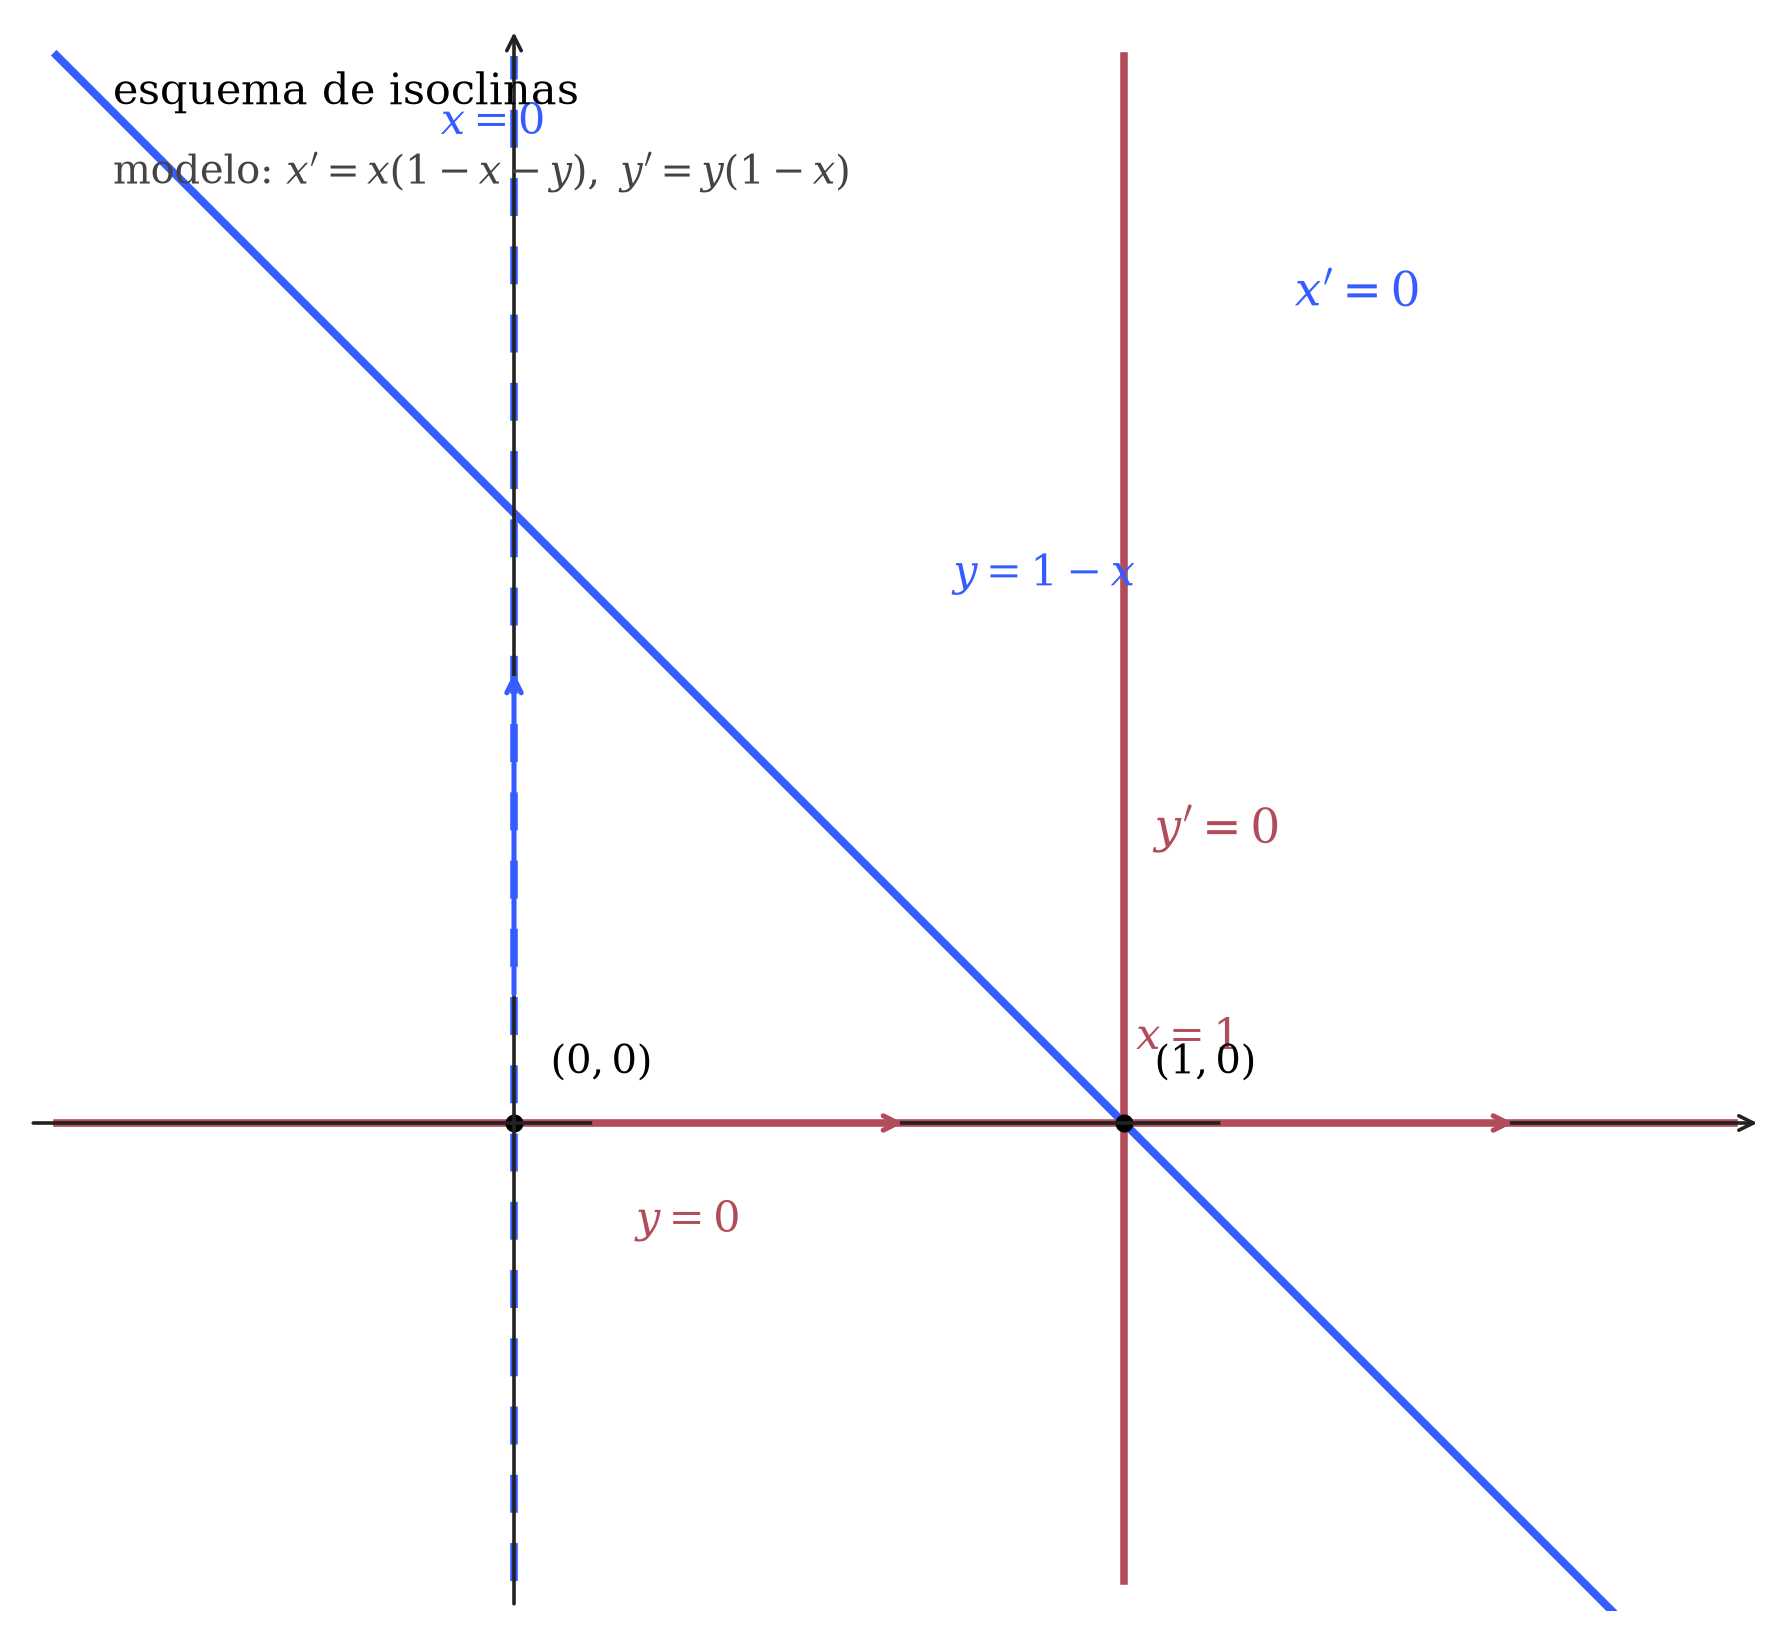
\includegraphics[width=0.92\linewidth]{fig_23_competencia_isoclinas.png}
\end{figure}

\begin{figure}[H]
\centering
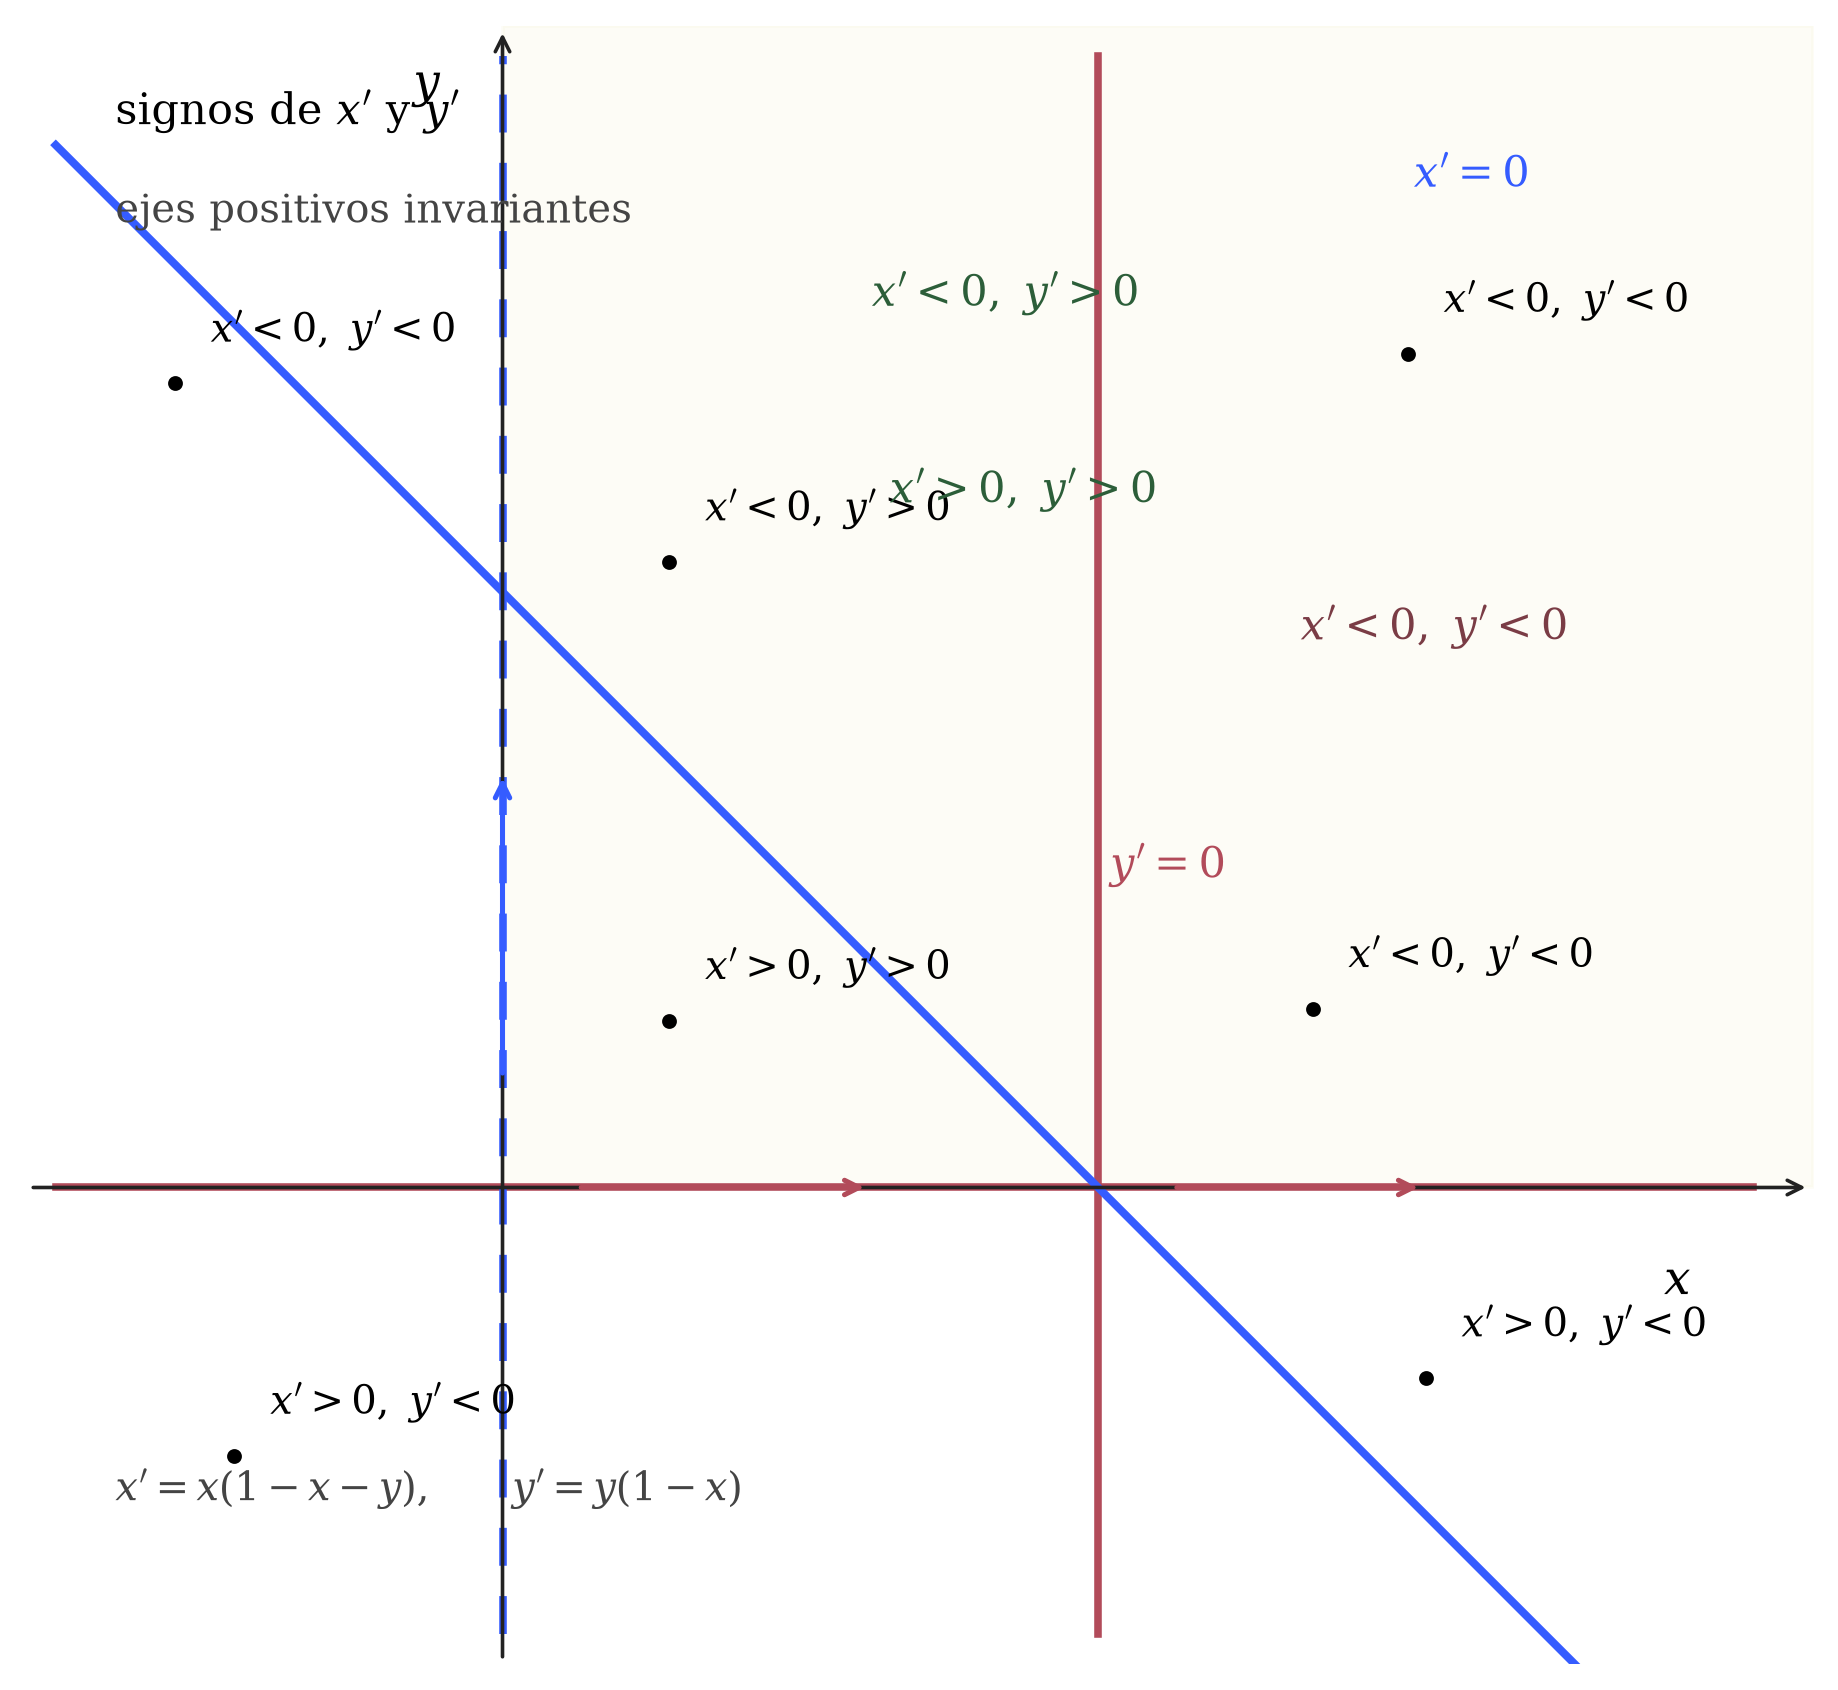
\includegraphics[width=0.92\linewidth]{fig_24_competencia_signos.png}
\end{figure}

\noindent Con esta informaci\'on se obtiene el esbozo del campo en el primer cuadrante.

\noindent \naglecite{cap.~5: el diagrama de fase se arma precisamente a partir de estas regiones de signo.}

\newpage
\textbf{Depredador-presa}

\noindent Dos poblaciones: presas \((P)\), depredadores \((D)\), distribuidos de manera uniforme en su h\'abitat.

\noindent \textbf{Hip\'otesis:}

\noindent I) En ausencia de depredador, la presa presenta crecimiento exponencial.

\[
\frac{dP}{dt}=\alpha P
\]

\noindent II) En ausencia de presa, el depredador se extingue exponencialmente.

\[
\frac{dD}{dt}=-\gamma D
\]

\noindent III) Cuando ambas poblaciones son positivas:

\[
\frac{dP}{dt}=\alpha P-\beta PD
\]

\[
\frac{dD}{dt}=-\gamma D+\delta PD
\]

\[
\alpha=\text{tasa intr\'inseca de crecimiento de la presa}
\]

\[
\gamma=\text{tasa intr\'inseca de muerte del depredador}
\]

\[
\beta=\text{tasa de muerte de la presa debida a encuentros con el depredador}
\]

\[
\delta=\text{tasa de aprovechamiento de la biomasa (presa) por el depredador}
\]

\noindent R\'otulos del esquema: \(P\) presas, \(D\) depredadores, Interacciones.

\begin{figure}[H]
\centering
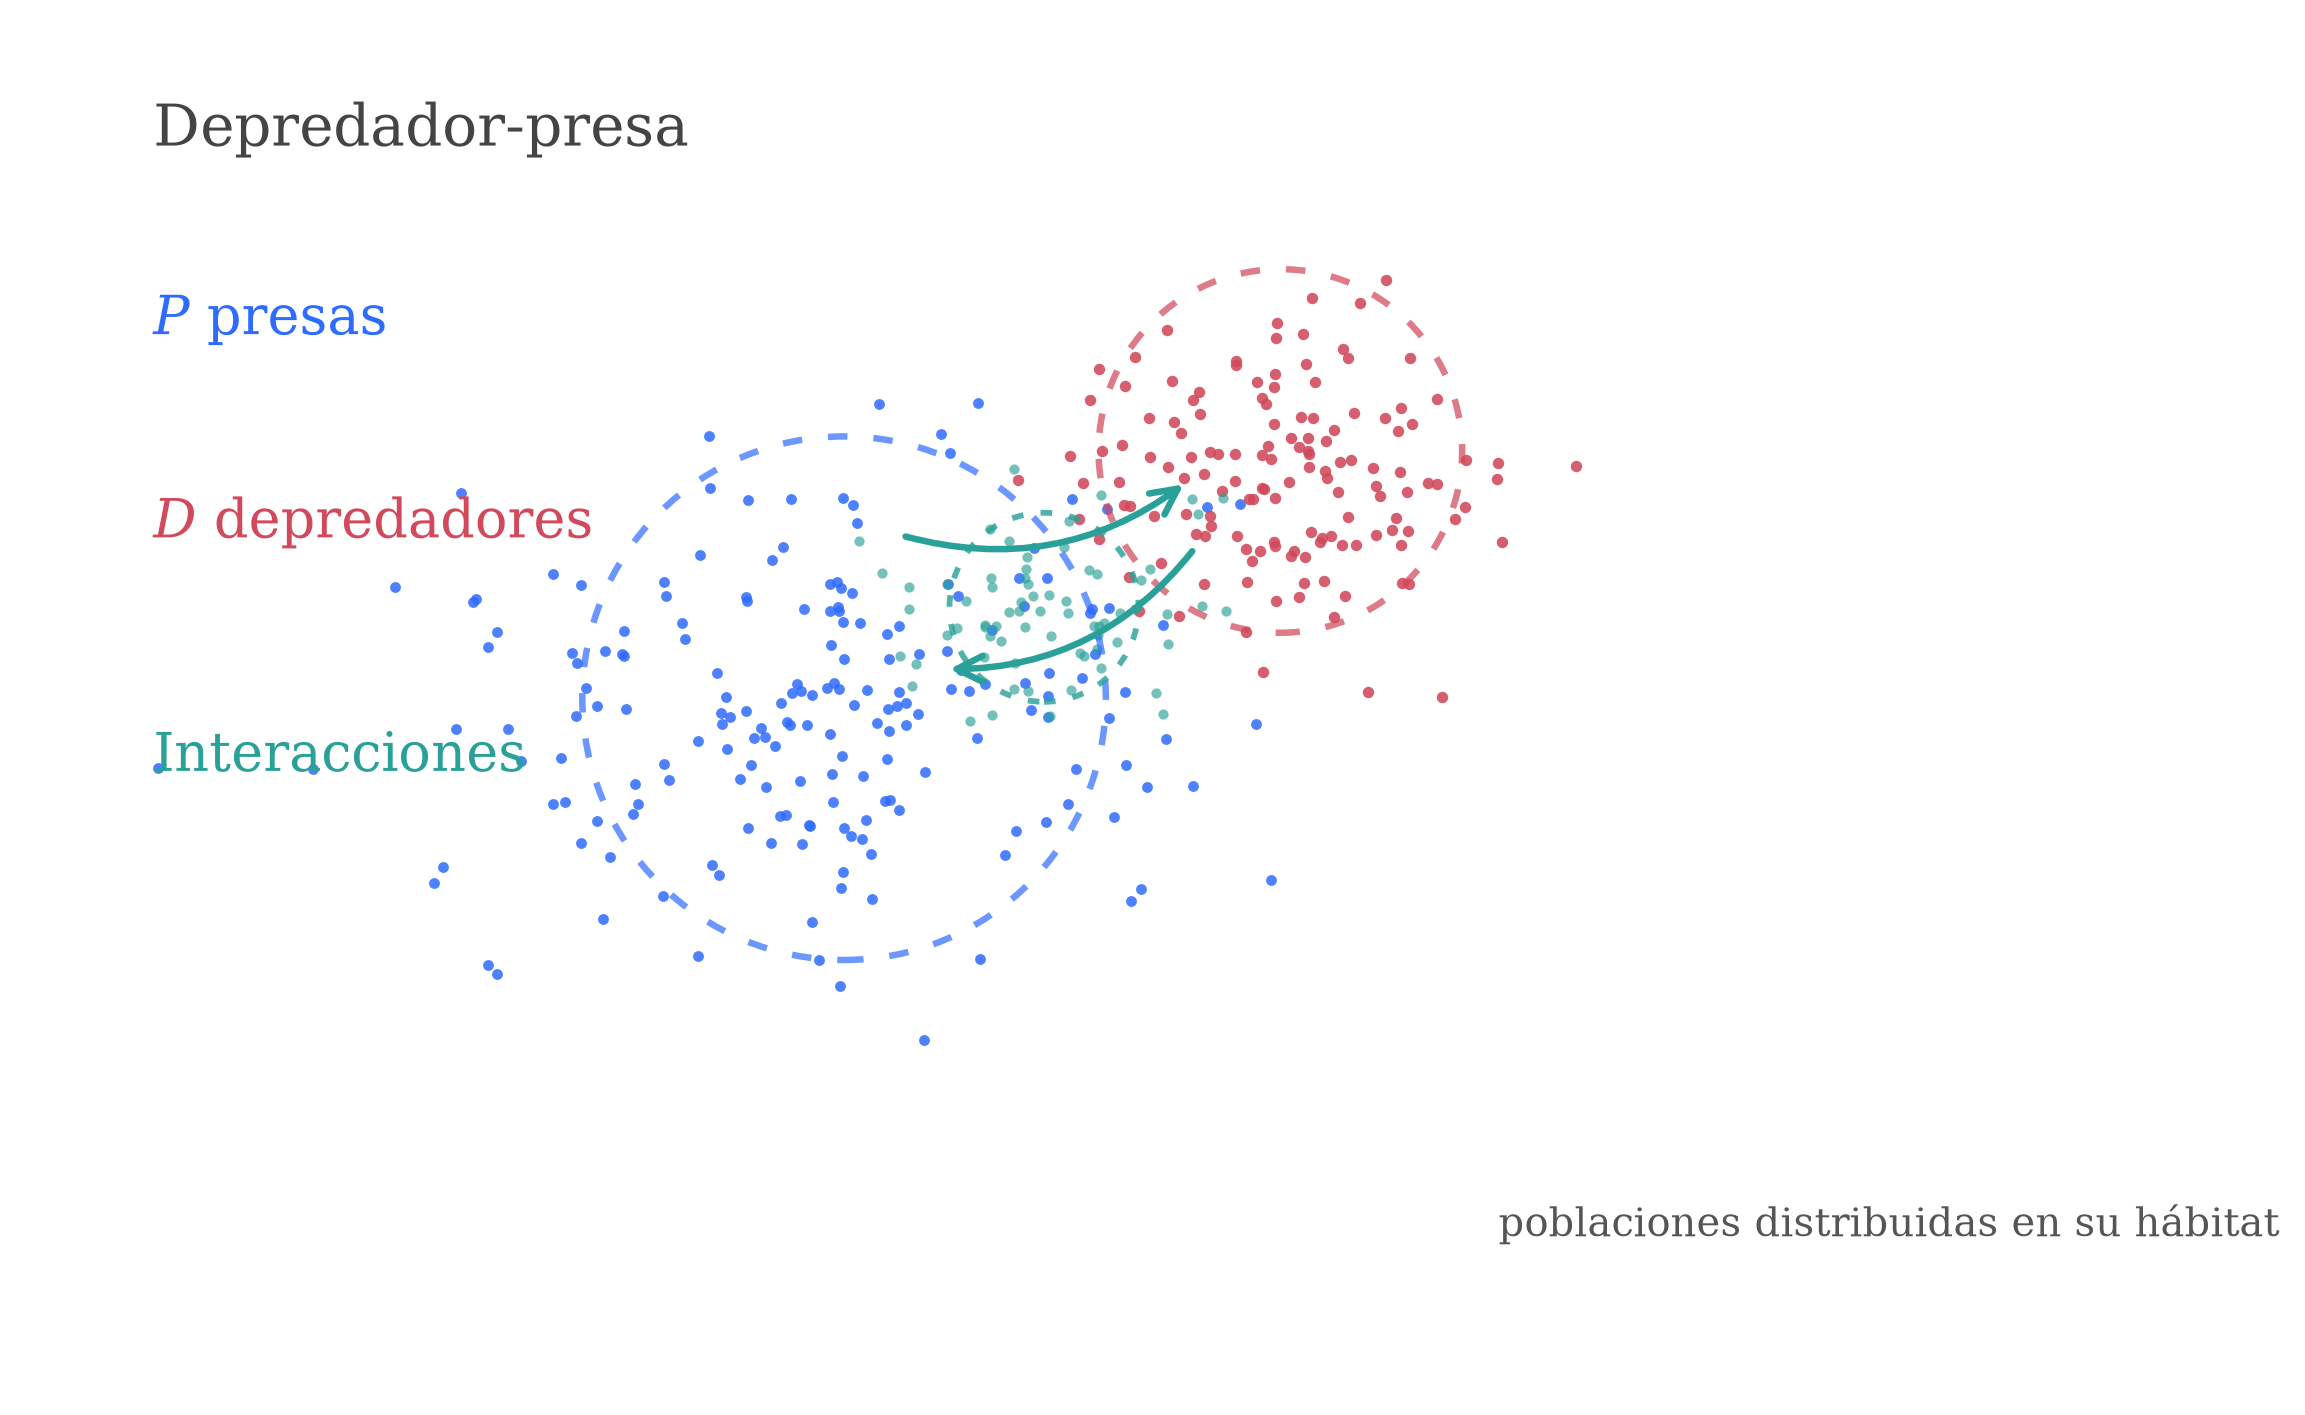
\includegraphics[width=0.92\linewidth]{fig_25_depredador_presa.png}
\end{figure}

\noindent \textbf{An\'alisis algebraico ordenado del modelo depredador-presa.}

\noindent Partimos del sistema de Lotka-Volterra

\[
P'=P(\alpha-\beta D), \qquad D'=D(\delta P-\gamma),
\]

\noindent donde \(P\) representa a las presas y \(D\) a los depredadores.
Como los factores \(P\) y \(D\) aparecen multiplicando, los ejes coordenados son invariantes:

\[
P=0 \Rightarrow P'=0 \Rightarrow \text{el eje }D\text{ es invariante},
\]

\[
D=0 \Rightarrow D'=0 \Rightarrow \text{el eje }P\text{ es invariante}.
\]

\noindent \textbf{1) Isoclinas nulas.}

\noindent Para \(P'\):

\[
P'=0 \iff P=0 \ \text{o} \ \alpha-\beta D=0 \iff D=\frac{\alpha}{\beta}.
\]

\noindent Para \(D'\):

\[
D'=0 \iff D=0 \ \text{o} \ \delta P-\gamma=0 \iff P=\frac{\gamma}{\delta}.
\]

\noindent Las rectas \(D=\alpha/\beta\) y \(P=\gamma/\delta\), junto con los ejes coordenados, particionan el plano en regiones.
La primera figura resume la informaci\'on geom\'etrica obtenida hasta este punto.

\noindent \naglecite{cap.~5: en modelos de competencia y depredador-presa, las nullclines organizan el plano fase.}

\noindent \textit{Descripci\'on de la figura 1:} se muestran los ejes invariantes, las isoclinas nulas
\(D=\alpha/\beta\) y \(P=\gamma/\delta\), y los puntos de equilibrio \(E_1=(0,0)\) y
\(E^*=(\gamma/\delta,\alpha/\beta)\). Esta imagen sirve para ubicar la estructura b\'asica del campo.

\begin{figure}[H]
\centering
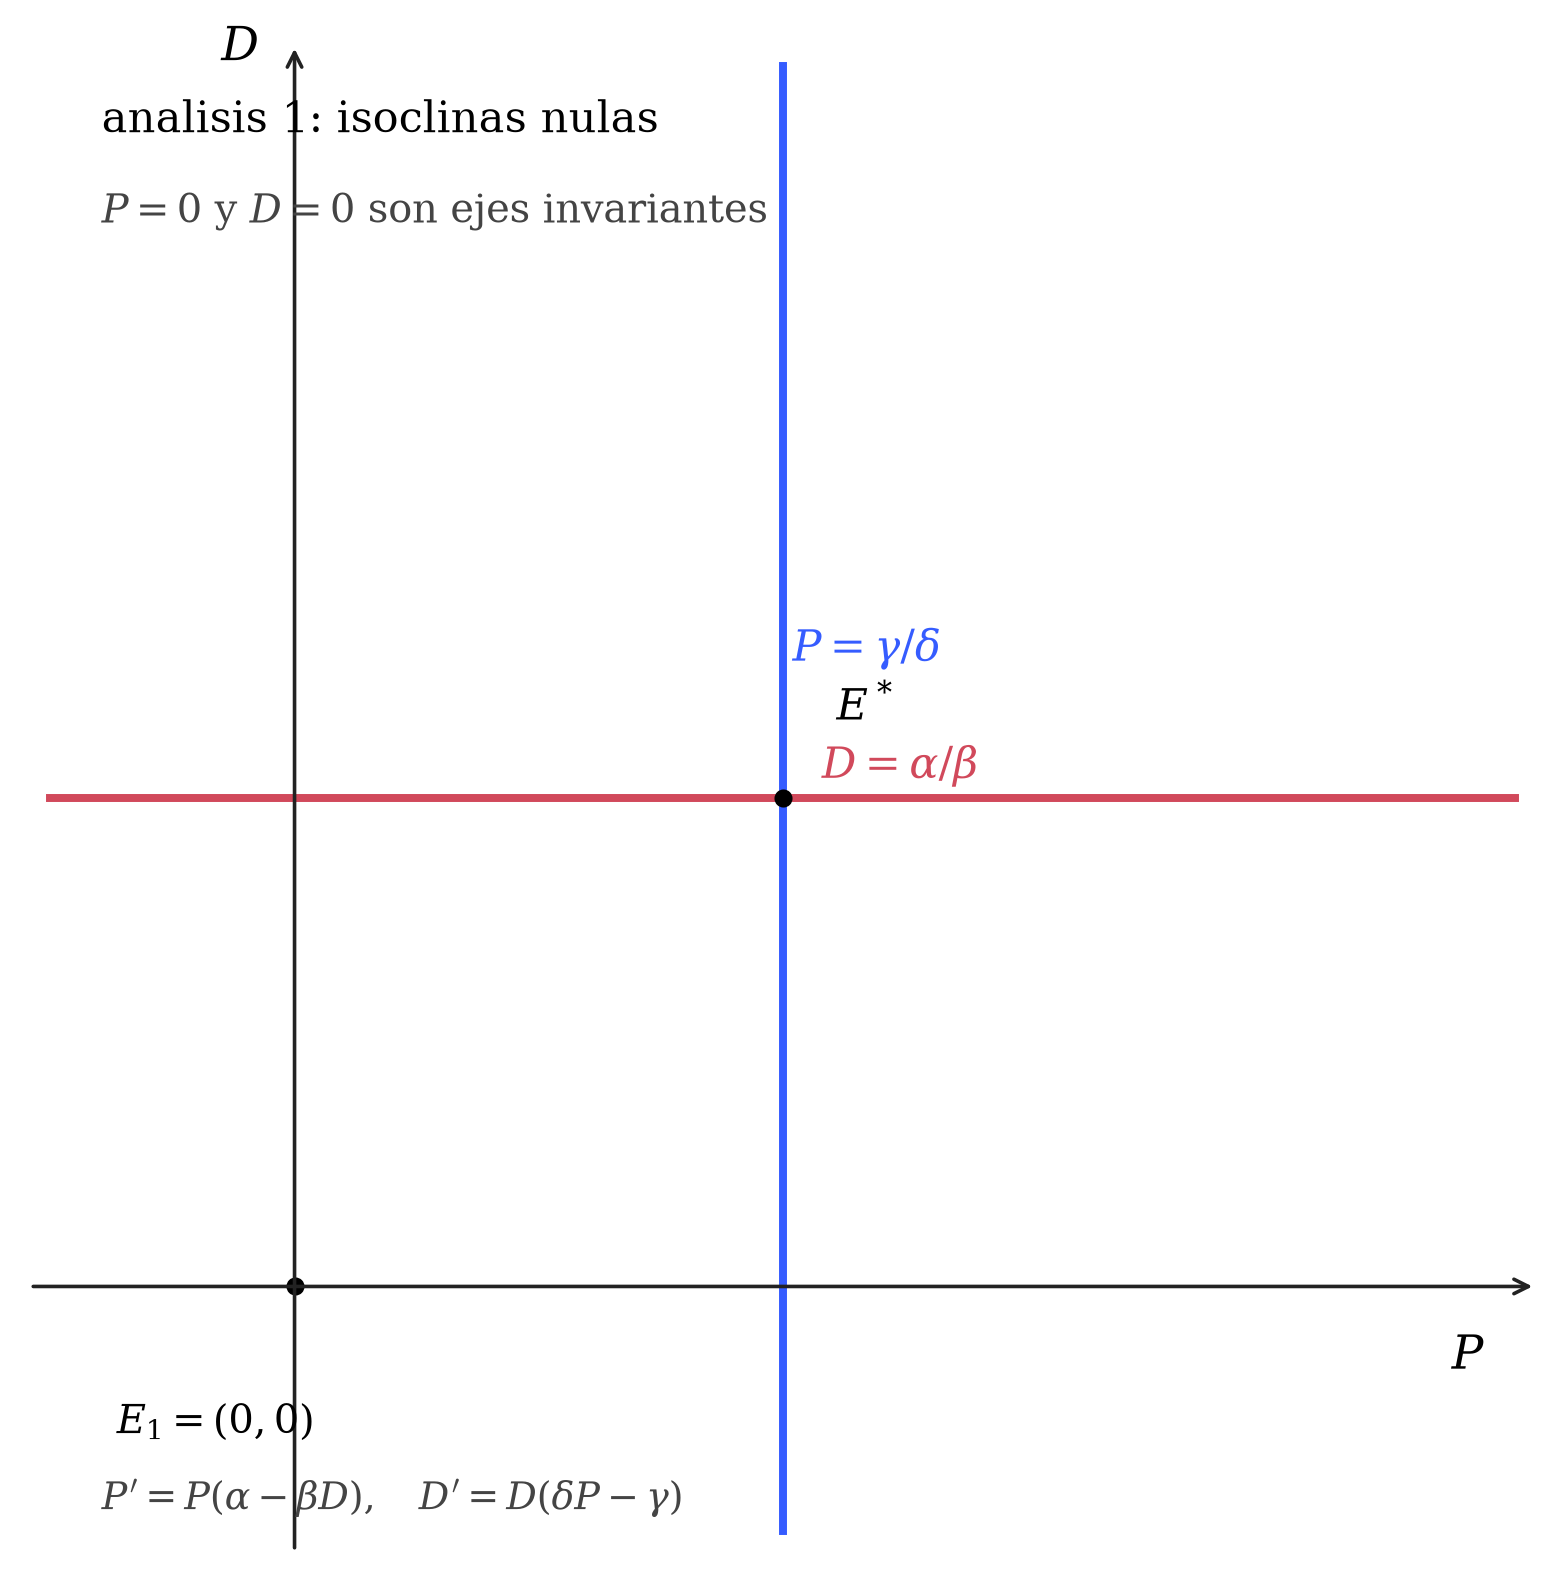
\includegraphics[width=0.92\linewidth]{fig_27_depredador_presa_etapa1.png}
\end{figure}

\noindent \textbf{2) An\'alisis de signos en el primer cuadrante.}

\noindent Desde el punto de vista biol\'ogico, el an\'alisis se restringe al primer cuadrante \(P\geq 0\), \(D\geq 0\).
Al comparar cada punto con las rectas \(D=\alpha/\beta\) y \(P=\gamma/\delta\), se obtienen los signos:

\[
0<P<\frac{\gamma}{\delta},\ 0<D<\frac{\alpha}{\beta}
\Rightarrow P'>0,\ D'<0,
\]

\[
0<P<\frac{\gamma}{\delta},\ D>\frac{\alpha}{\beta}
\Rightarrow P'<0,\ D'<0,
\]

\[
P>\frac{\gamma}{\delta},\ 0<D<\frac{\alpha}{\beta}
\Rightarrow P'>0,\ D'>0,
\]

\[
P>\frac{\gamma}{\delta},\ D>\frac{\alpha}{\beta}
\Rightarrow P'<0,\ D'>0.
\]

\noindent Con esta informaci\'on se determina la direcci\'on del flujo en cada subregi\'on y, con ello, se bosqueja el comportamiento global.

\noindent \naglecite{cap.~5 y cap.~12: el plano fase y la estabilidad local se leen a partir de las nullclines y del jacobiano.}

\noindent \textit{Descripci\'on de la figura 2:} se agregan los signos de \(P'\) y \(D'\) en cada regi\'on del primer cuadrante,
as\'i como las flechas de direcci\'on del flujo. La figura muestra c\'omo el plano se organiza alrededor de las isoclinas nulas.

\begin{figure}[H]
\centering
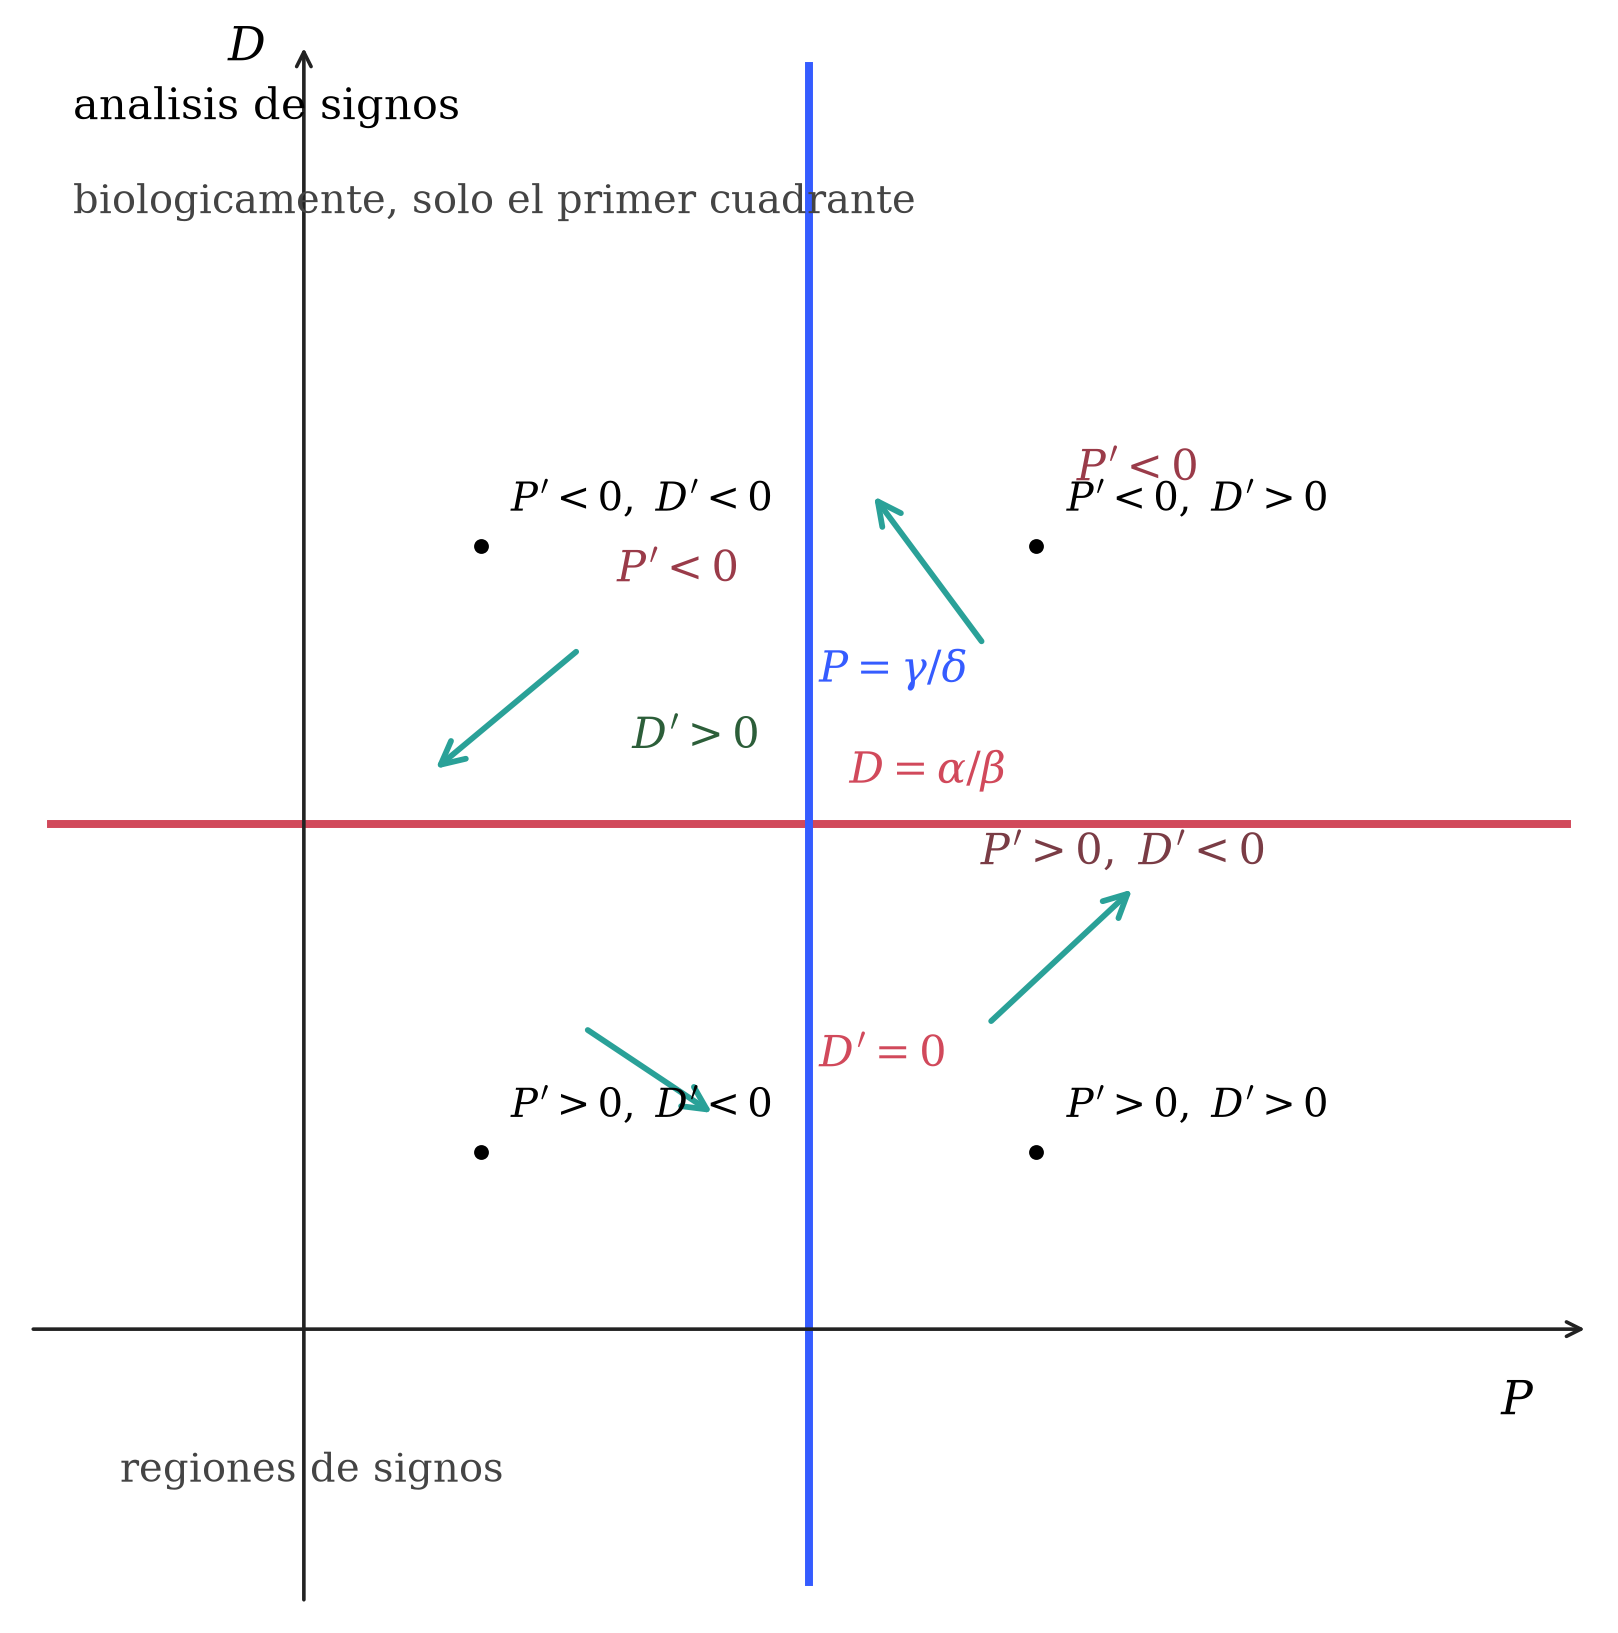
\includegraphics[width=0.92\linewidth]{fig_28_depredador_presa_etapa2.png}
\end{figure}

\noindent \textbf{3) Puntos de equilibrio y estabilidad local.}

\noindent El jacobiano del sistema es

\[
J(P,D)=
\begin{pmatrix}
\alpha-\beta D & -\beta P \\
\delta D & \delta P-\gamma
\end{pmatrix}.
\]

\noindent En el equilibrio de extinci\'on \(E_1=(0,0)\) se obtiene

\[
J(E_1)=
\begin{pmatrix}
\alpha & 0 \\
0 & -\gamma
\end{pmatrix}.
\]

\noindent Sus valores propios son \(\lambda_1=\alpha\) y \(\lambda_2=-\gamma\), por lo que \(E_1\) es hiperb\'olico y de tipo silla.
Por el teorema de Hartman-Grobman, el retrato local es topol\'ogicamente equivalente al del sistema lineal asociado.

\noindent En el equilibrio de coexistencia

\[
E^*=\left(\frac{\gamma}{\delta},\frac{\alpha}{\beta}\right),
\]

\noindent se tiene

\[
J(E^*)=
\begin{pmatrix}
0 & -\beta\left(\frac{\gamma}{\delta}\right) \\
\delta\left(\frac{\alpha}{\beta}\right) & 0
\end{pmatrix}.
\]

\noindent El polinomio caracter\'istico es

\[
\lambda^2+\alpha\gamma=0,
\]

\noindent de donde

\[
\lambda=\pm i\sqrt{\alpha\gamma}.
\]

\noindent Por tanto, \(E^*\) no es hiperb\'olico; en el modelo cl\'asico de Lotka-Volterra las trayectorias alrededor de este punto se cierran.

\noindent \naglecite{cap.~12: la linealizaci\'on explica el comportamiento local cerca de los puntos cr\'iticos hiperb\'olicos.}

\noindent \textit{Descripci\'on de la figura 3:} se presenta el retrato local en el primer cuadrante, con
\(E_1\) como silla y \(E^*\) organizando las \'orbitas alrededor de la coexistencia.
Esta es la versi\'on final del esbozo del campo una vez que se integran las isoclinas, los signos y la estabilidad local.

\begin{figure}[H]
\centering
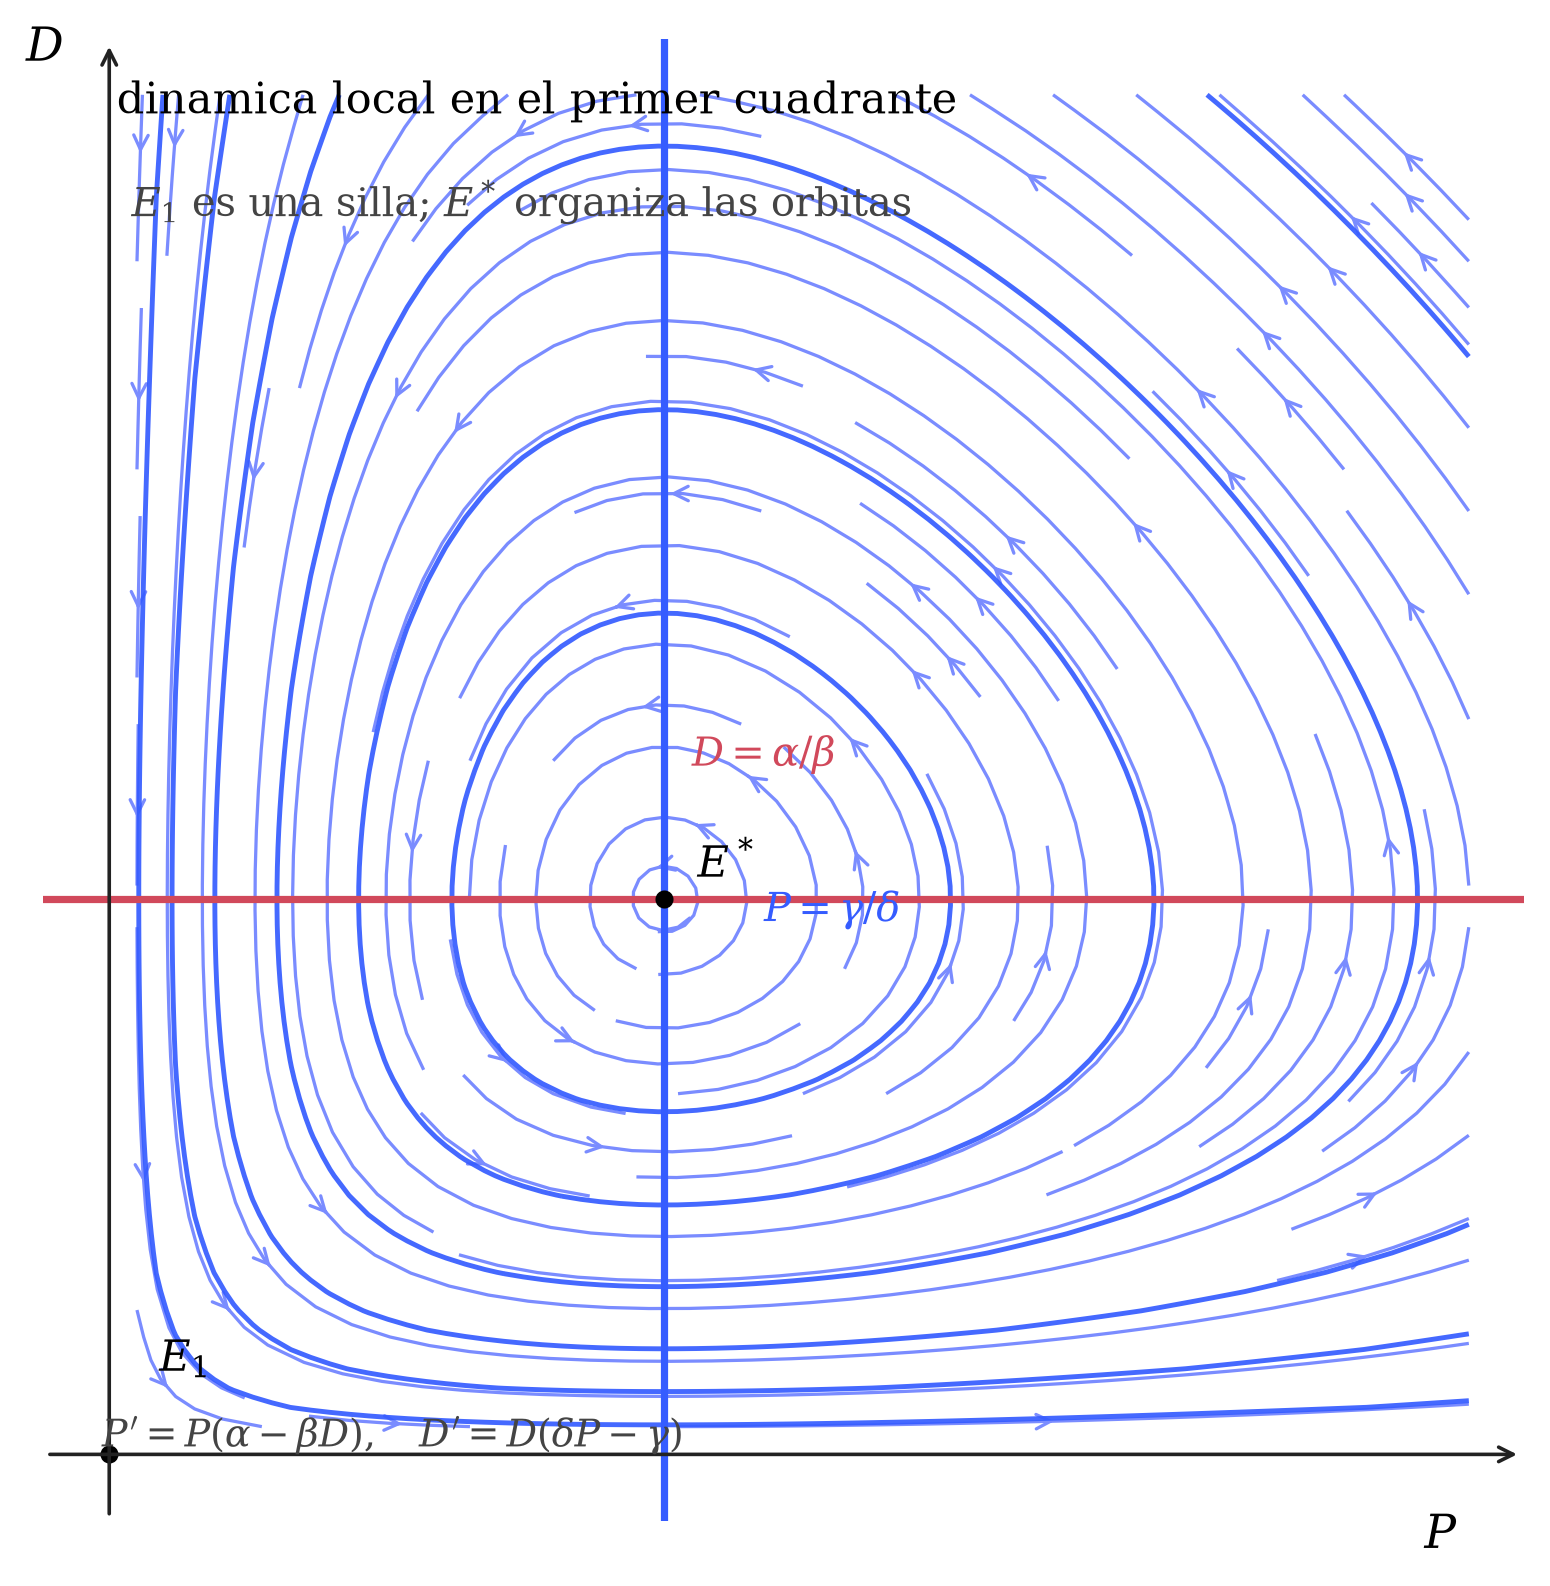
\includegraphics[width=0.92\linewidth]{fig_29_depredador_presa_etapa3.png}
\end{figure}

\noindent \textbf{Modelo de dos especies en competencia: \(N_1\) y \(N_2\)}

\noindent \textit{Primer modelo: crecimiento poblacional multiplicativo.}

\[
\begin{cases}
\dfrac{dN_1}{dt}=r_1N_1-\beta N_1N_2,\\[4pt]
\dfrac{dN_2}{dt}=r_2N_2-\delta N_1N_2.
\end{cases}
\]

\noindent \textit{Segundo modelo: crecimiento log\'istico.}

\[
\begin{cases}
\dfrac{dN_1}{dt}=r_1N_1\left(1-\dfrac{N_1}{K_1}\right)-\beta N_1N_2,\\[4pt]
\dfrac{dN_2}{dt}=r_2N_2\left(1-\dfrac{N_2}{K_2}\right)+\delta N_1N_2.
\end{cases}
\]

\noindent \textbf{Ejemplo algebraico.}

\[
\frac{dx}{dt}=-3x+4xy-3x^2
\]

\[
\frac{dy}{dt}=2y-3xy-0.5y^2
\]

\noindent \textbf{Una segunda v\'ia para obtener informaci\'on cualitativa.}

\noindent Tomamos el campo vectorial

\[
F(P,D)=
\begin{pmatrix}
P(\alpha-\beta D)\\
D(-\gamma+\delta P)
\end{pmatrix}.
\]

\noindent En la regi\'on biol\'ogicamente relevante \(P,D>0\), podemos escribir

\[
\frac{dD}{dP}=\frac{D(-\gamma+\delta P)}{P(\alpha-\beta D)}.
\]

\noindent Separando variables,

\[
\left(\frac{-\gamma+\delta P}{P}\right)dP=\left(\frac{\alpha-\beta D}{D}\right)dD.
\]

\noindent Luego,

\[
\int\left(-\frac{\gamma}{P}+\delta\right)dP=\int\left(\frac{\alpha}{D}-\beta\right)dD.
\]

\[
-\gamma\ln P+\delta P=\alpha\ln D-\beta D+C.
\]

\noindent En consecuencia, una integral primera para el sistema queda dada por

\[
H(P,D)=-\gamma\ln P+\delta P+\beta D-\alpha\ln D.
\]

\noindent En consecuencia,

\[
H(P,D)=\mathrm{cte.}
\]

\noindent y sus curvas de nivel son las \'orbitas del sistema.

\noindent \textit{Descripci\'on de la figura 4:} se resume la deducci\'on algebraica de la integral primera a partir de
\(\frac{dD}{dP}\), la separaci\'on de variables y la expresi\'on final de \(H(P,D)\).
Esta imagen sirve como puente entre el an\'alisis de signos y el comportamiento global del sistema.

\begin{figure}[H]
\centering

\includegraphics[width=0.92\linewidth]{fig_32_depredador_presa_integral_derivacion.png}
\end{figure}

\noindent \textit{Descripci\'on de la figura 5:} el campo vectorial en el primer cuadrante se dibuja junto con las curvas de nivel de
\(H(P,D)\). Se distinguen los ejes invariantes, el equilibrio \(E_1=(0,0)\), el equilibrio de coexistencia
\(E^*=(\gamma/\delta,\alpha/\beta)\) y las \'orbitas cerradas alrededor de \(E^*\).

\begin{figure}[H]
\centering
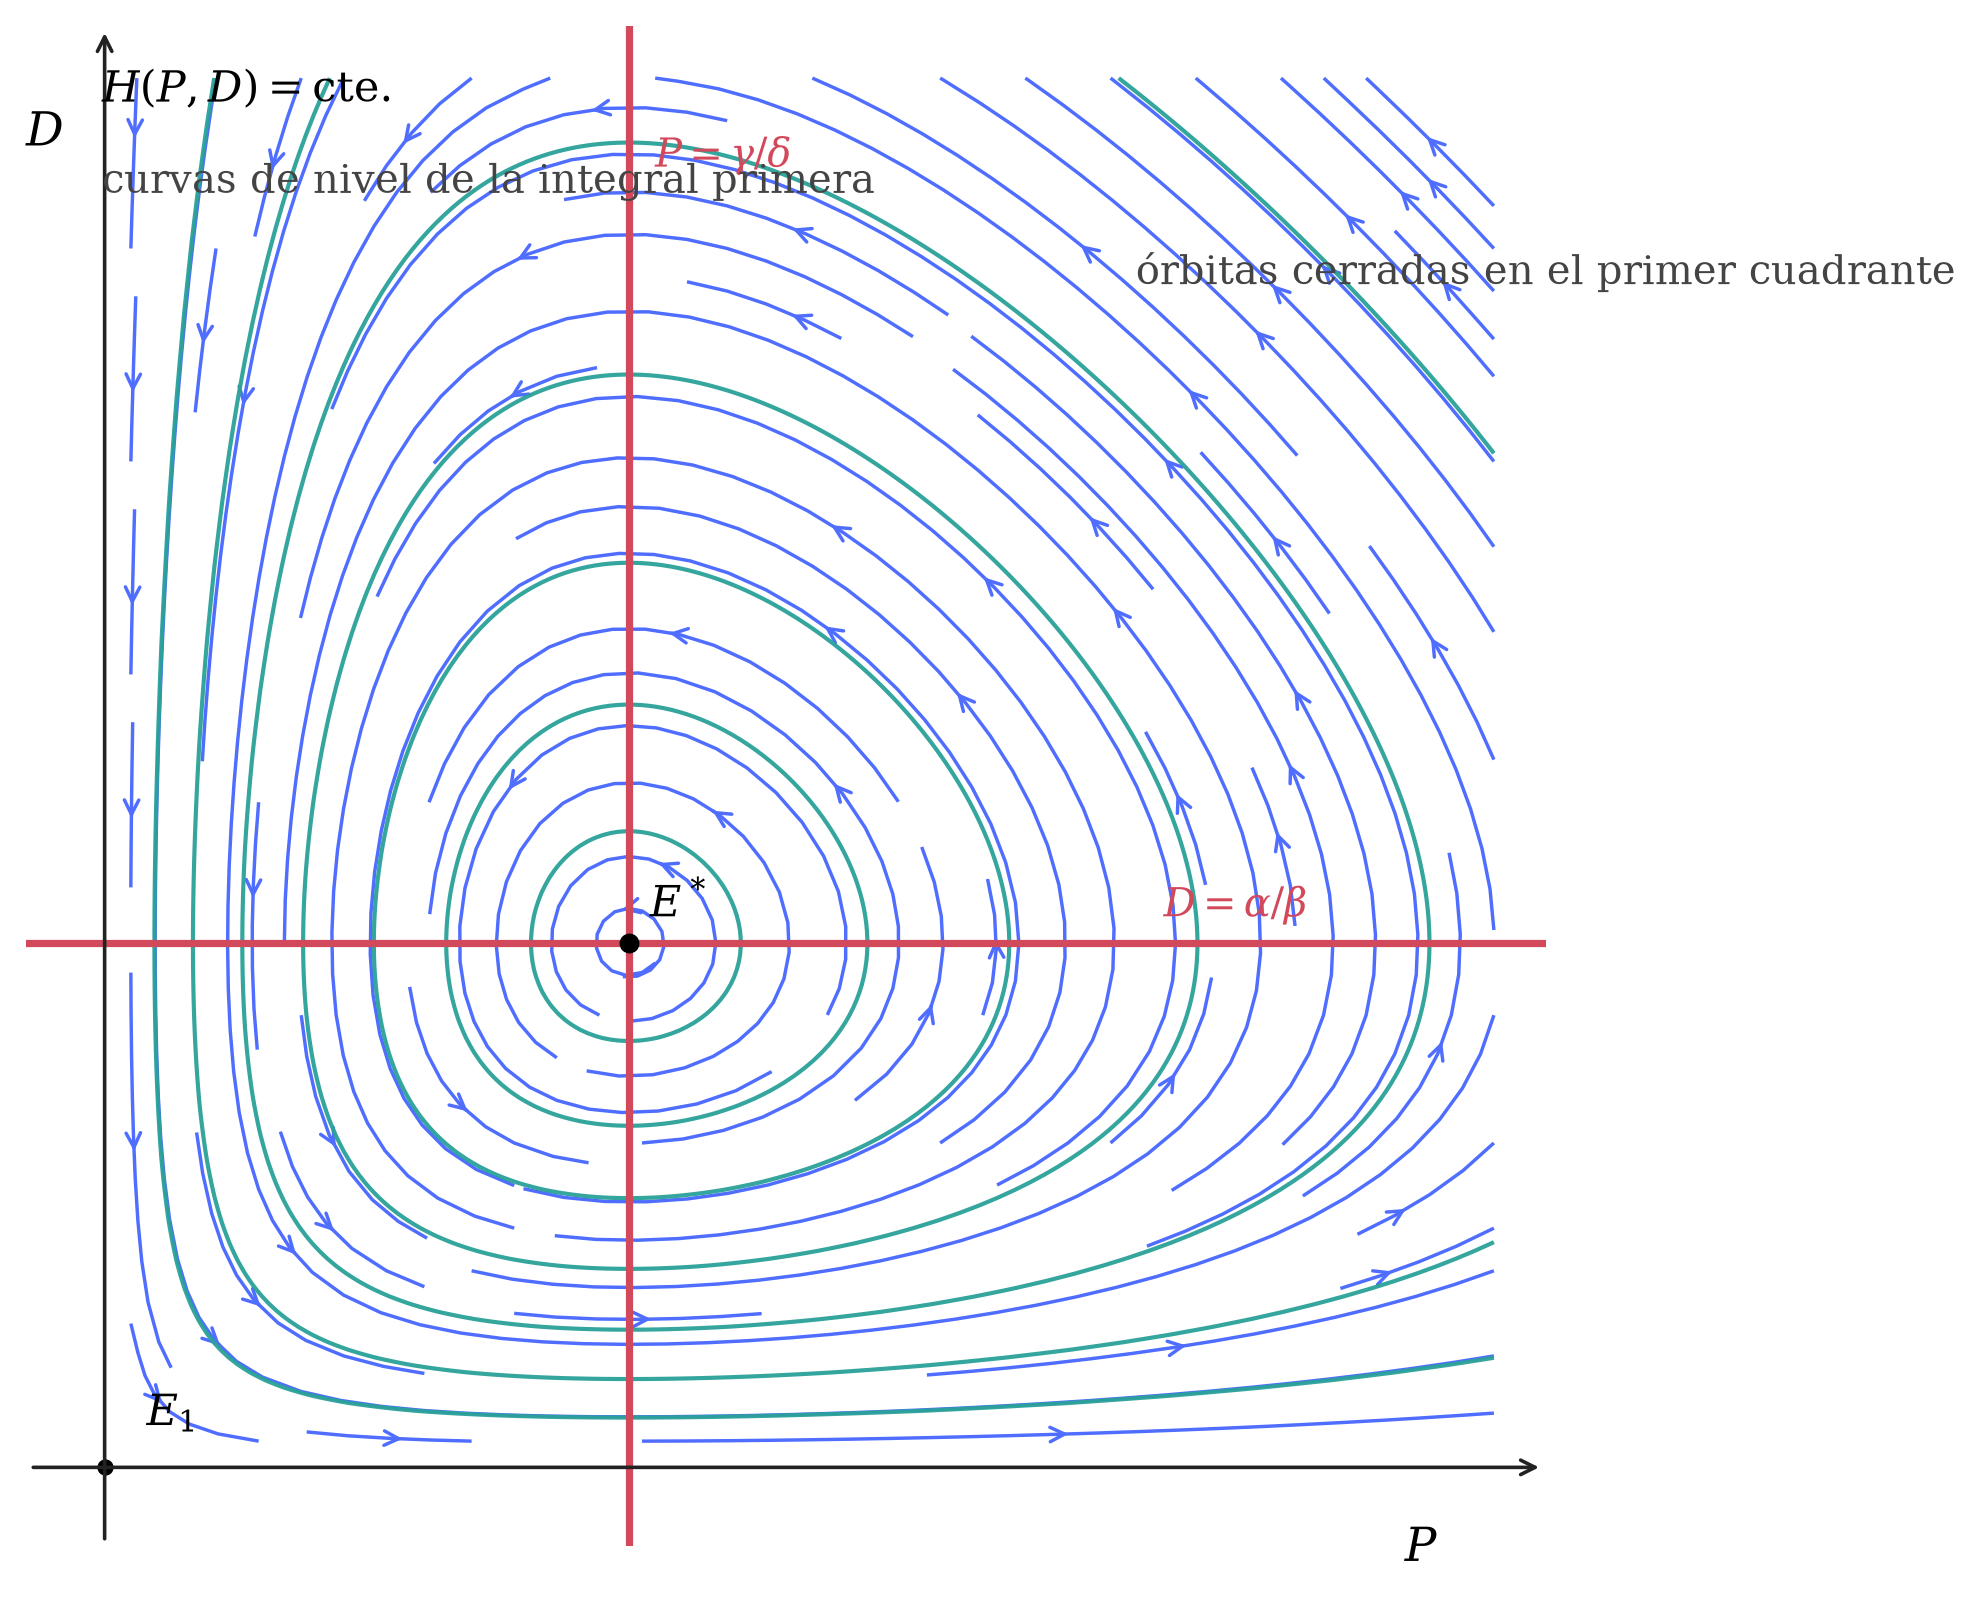
\includegraphics[width=0.92\linewidth]{fig_33_depredador_presa_integral_orbitas.png}
\end{figure}

\newpage
\textbf{Sistema de tres variables}

\[
x_1'=x_1\,f_1(x_1,x_2,x_3)
\]

\[
x_2'=x_2\,f_2(x_1,x_2,x_3)
\]

\[
x_3'=x_3\,f_3(x_1,x_2,x_3)
\]

\[
x_1=0 \Rightarrow x_1'=0 \Rightarrow \text{plano } x_2x_3 \text{ es invariante}
\]

\[
x_2=0 \Rightarrow x_2'=0 \Rightarrow \text{plano } x_1x_3 \text{ es invariante}
\]

\[
x_3=0 \Rightarrow x_3'=0 \Rightarrow \text{plano } x_1x_2 \text{ es invariante}
\]

\[
\text{Por consiguiente, el primer octante es invariante.}
\]

\noindent \naglecite{cap.~12: en sistemas de mayor dimensi\'on, los subespacios invariantes simplifican el an\'alisis.}

\begin{figure}[H]
\centering
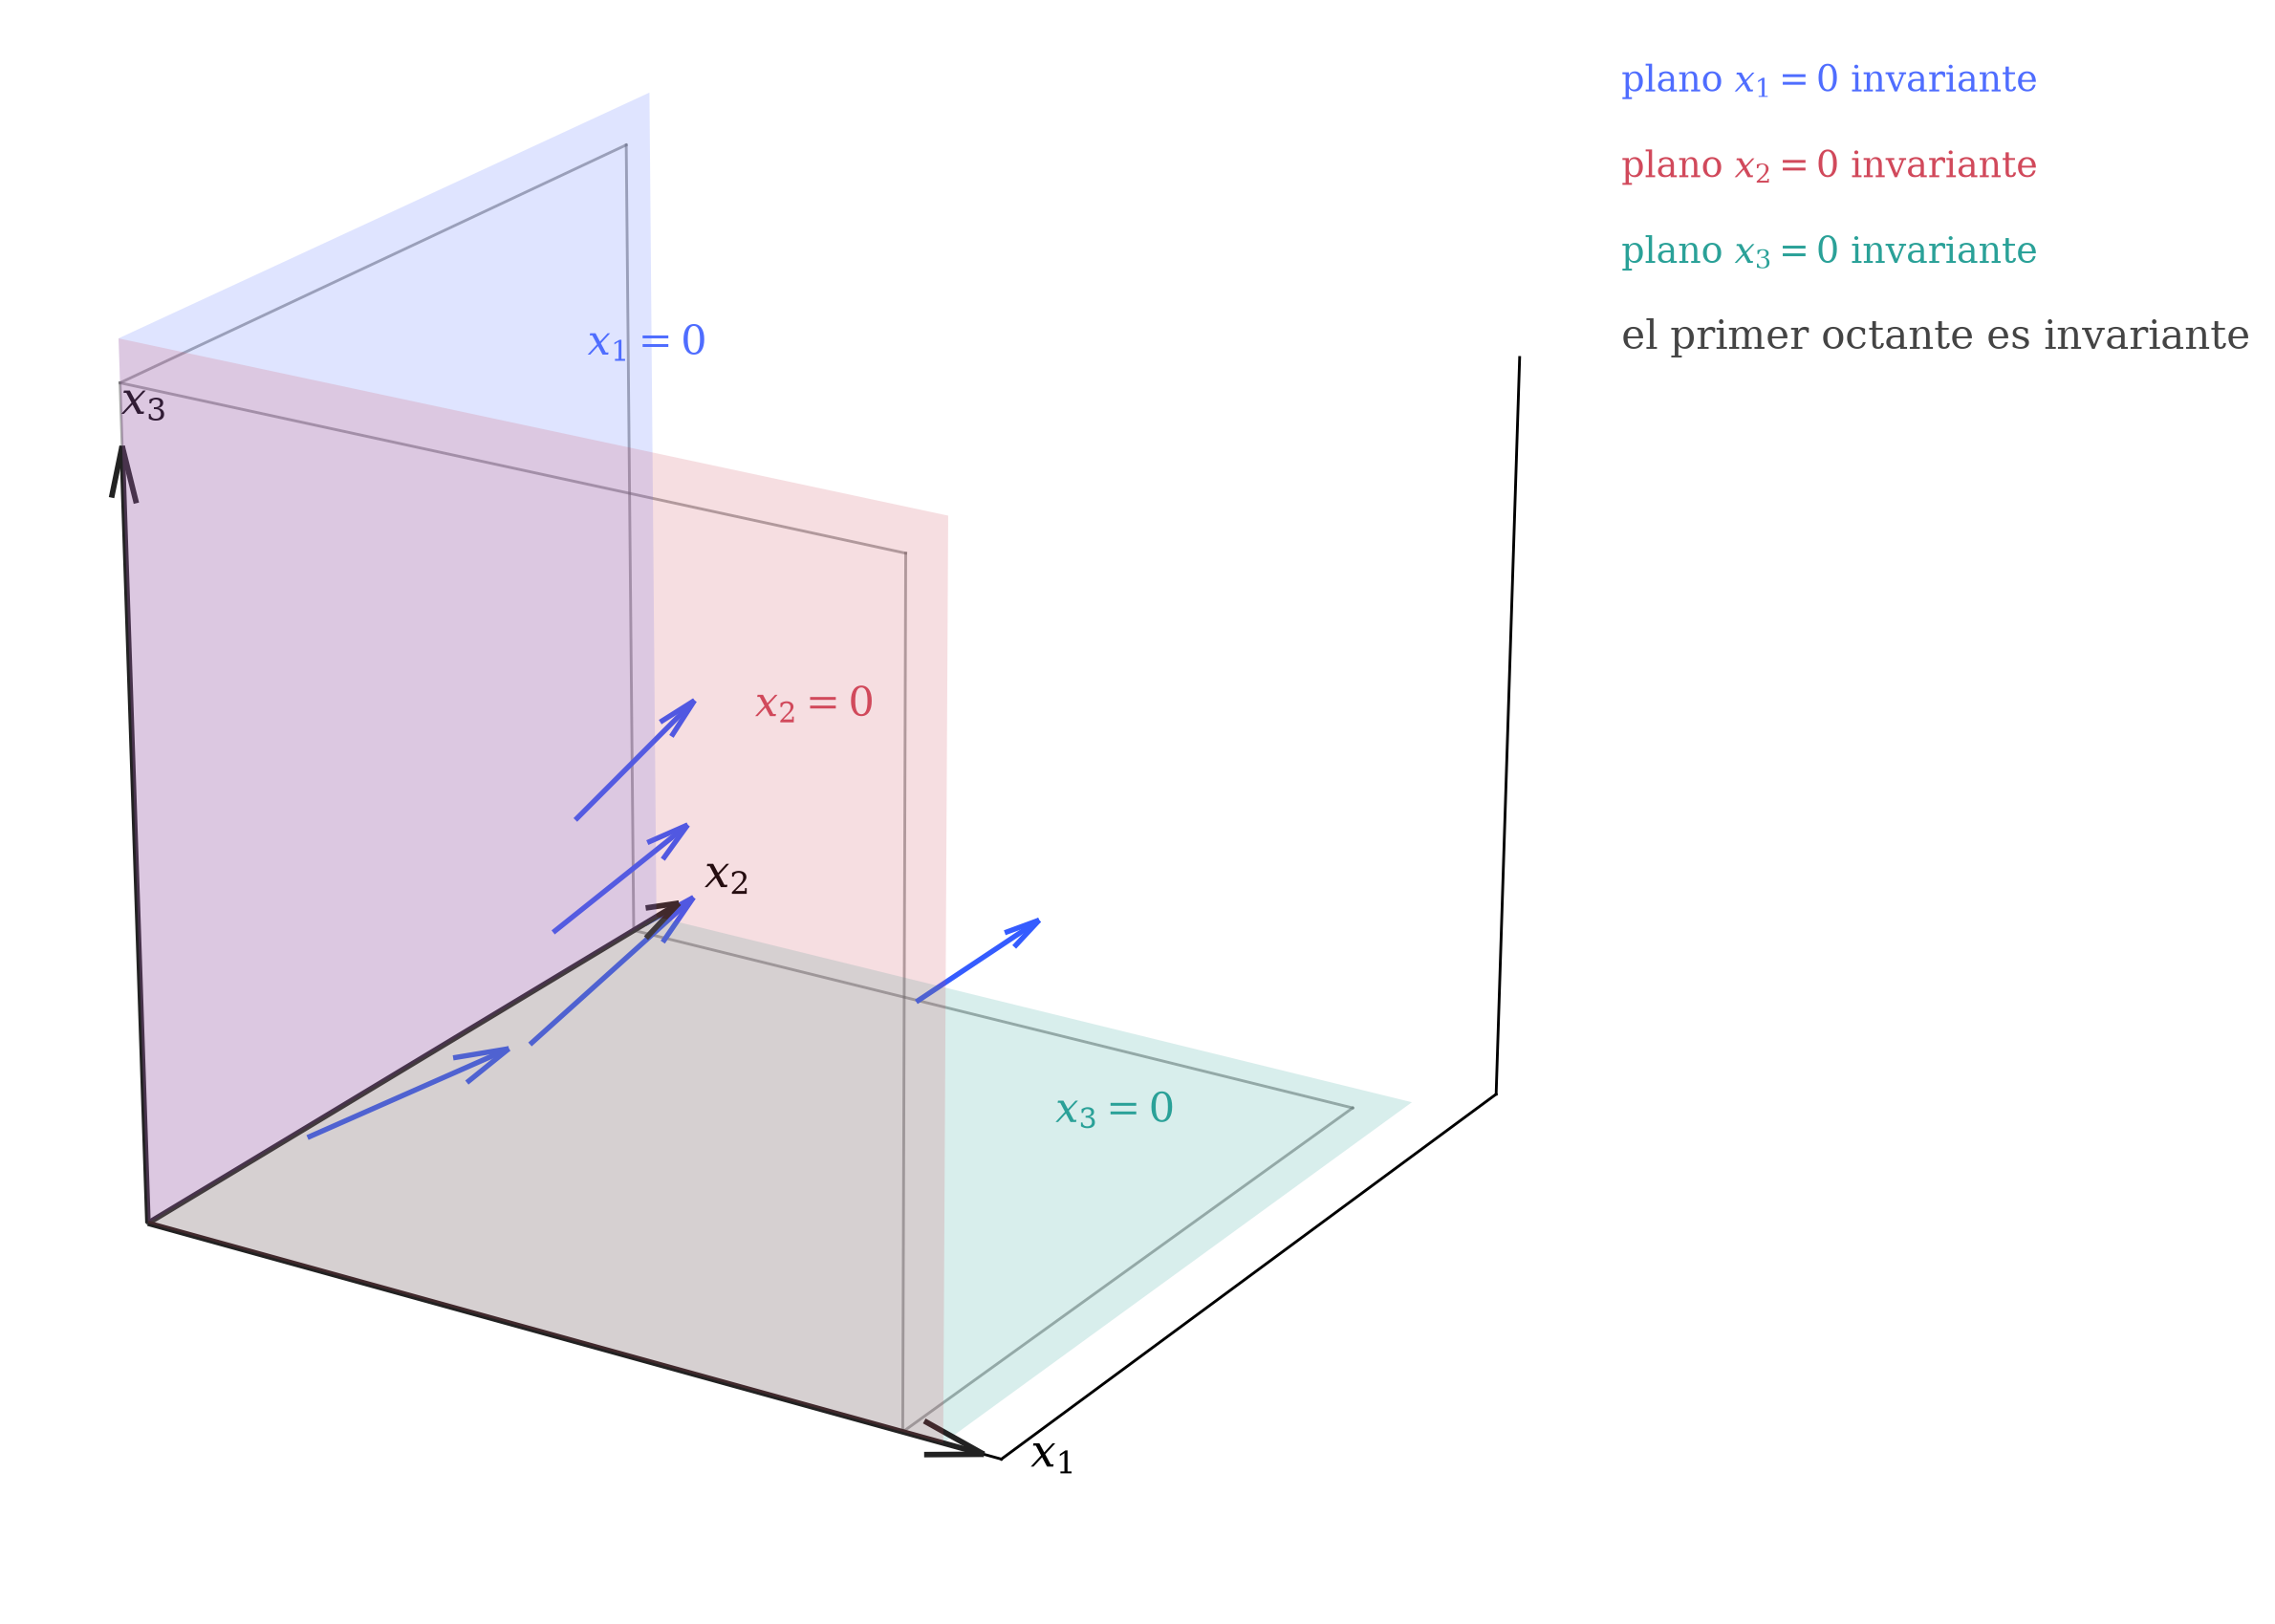
\includegraphics[width=0.92\linewidth]{fig_26_octante_invariante.png}
\end{figure}

\newpage
\textbf{Polinomio caracter\'istico e integrales primeras}

\noindent El polinomio caracter\'istico de \(DF(E^*)\) es

\[
p(\lambda)=\lambda^2+\beta\left(\frac{\gamma}{\delta}\right)\left(\frac{\alpha}{\beta}\right)\delta
=\lambda^2+\alpha\gamma.
\]

\noindent Tiene ra\'ices imaginarias puras.

\noindent Hartman-Grobman no es aplicable.

\noindent \textbf{Integrales primeras:}

\noindent Consideremos \(X'=F(X)\) en \(\mathbb{R}^n\).

\noindent \(F\) suficientemente diferenciable.

\noindent Una integral primera de \((*)\) es una funci\'on

\[
H:\mathbb{R}^n \to \mathbb{R}
\]

\noindent tal que si \(X(t)\) es soluci\'on de \((*)\), entonces \(H\) es constante a lo largo de \(X(t)\).

\noindent En particular,

\[
H(X(t))=\mathrm{cte.}
\]

\[
0=\frac{d}{dt}H(X(t))
=\nabla H(X(t))\cdot X'(t)
=\nabla H(X(t))\cdot F(X(t)).
\]

\noindent \textit{Interpretaci\'on:} el gradiente de \(H\), evaluado en \(X(t)\), es ortogonal al campo vectorial \(F(X(t))\).

\noindent \naglecite{cap.~12: este tipo de identidad se relaciona con argumentos de energ\'ia y con la geometr\'ia del flujo.}

\noindent \textit{Descripci\'on de la figura 1:} se muestran curvas de nivel de \(H\), una trayectoria \(X(t)\) sobre una de esas curvas, el vector \(F(X(t))\) tangente a la trayectoria y el vector \(\nabla H(X(t))\) perpendicular a ella. La idea central es que \(H(X(t))\) permanece constante a lo largo del flujo.

\begin{figure}[H]
\centering
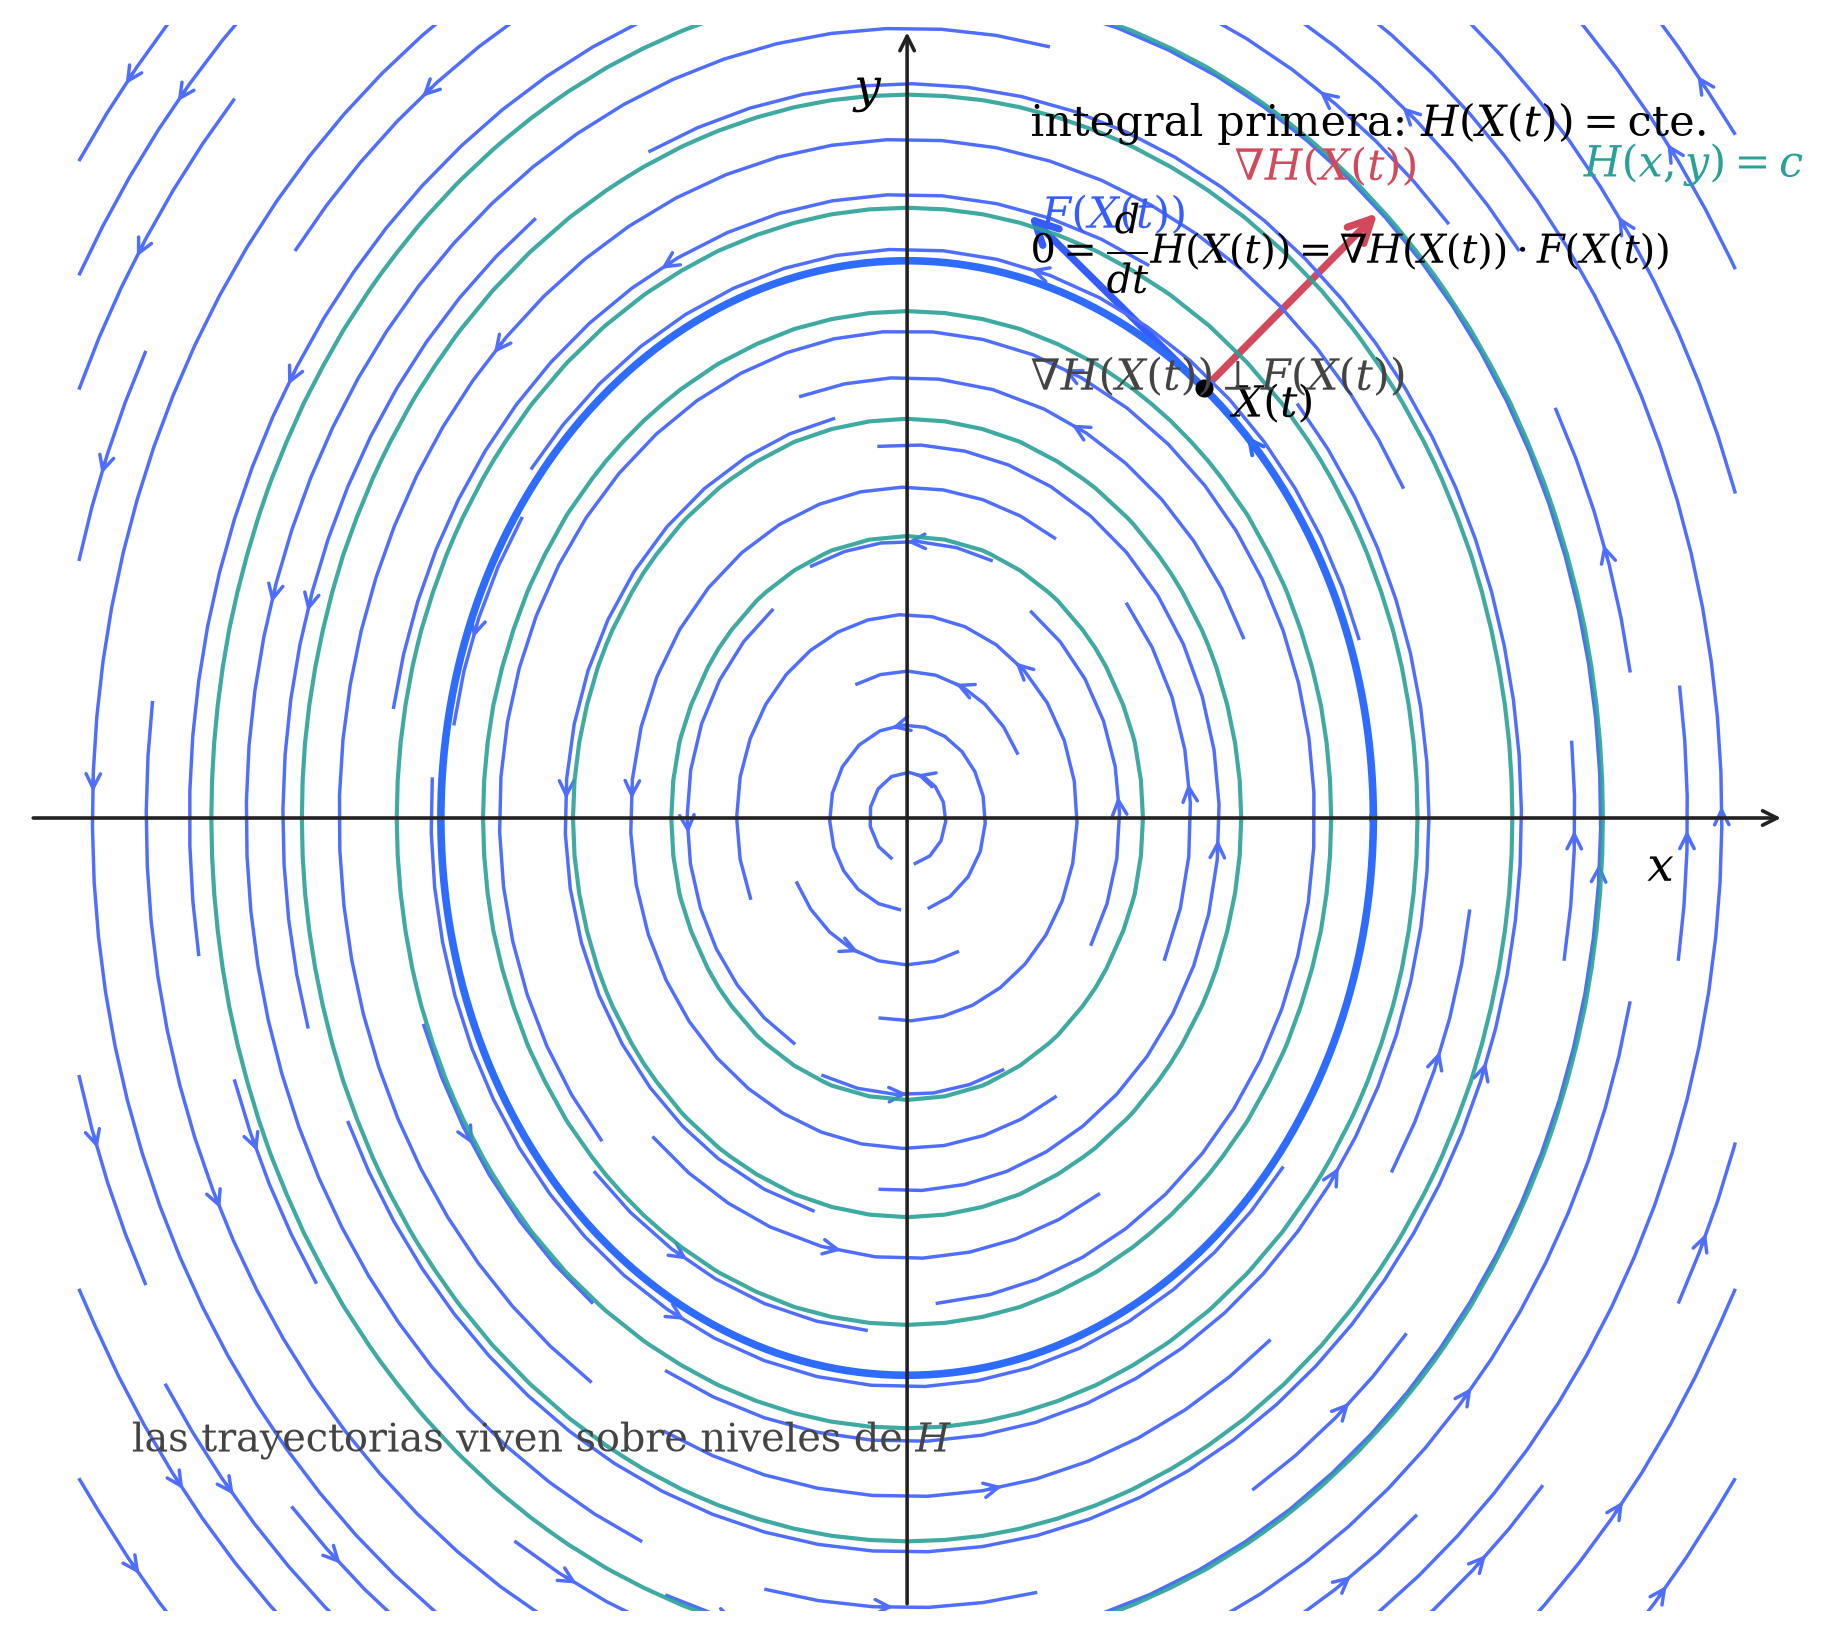
\includegraphics[width=0.92\linewidth]{fig_30_integral_primera_esquema.png}
\end{figure}

\noindent \textbf{Ejemplo con cosecha constante:}

\noindent Consideremos un modelo log\'istico con cosecha constante.

\[
X'=F(x,\mu),
\]

\noindent En particular,

\[
p'=\alpha p\left(1-\frac{p}{k}\right)-H.
\]

\noindent Definamos tambi\'en la funci\'on

\[
f(x)=\alpha x\left(1-\frac{x}{k}\right).
\]

\noindent \textit{Descripci\'on de la figura 2:} en el panel izquierdo se ve la curva de crecimiento log\'istico \(f(p)\) y la recta horizontal de cosecha \(H\); en el panel derecho se muestra la funci\'on neta \(p'=f(p)-H\), con sus intervalos de signo y los puntos donde cambia de positivo a negativo.

\noindent \naglecite{cap.~5: comparar la funci\'on neta con sus ceros es una forma directa de leer la din\'amica cualitativa.}

\begin{figure}[H]
\centering
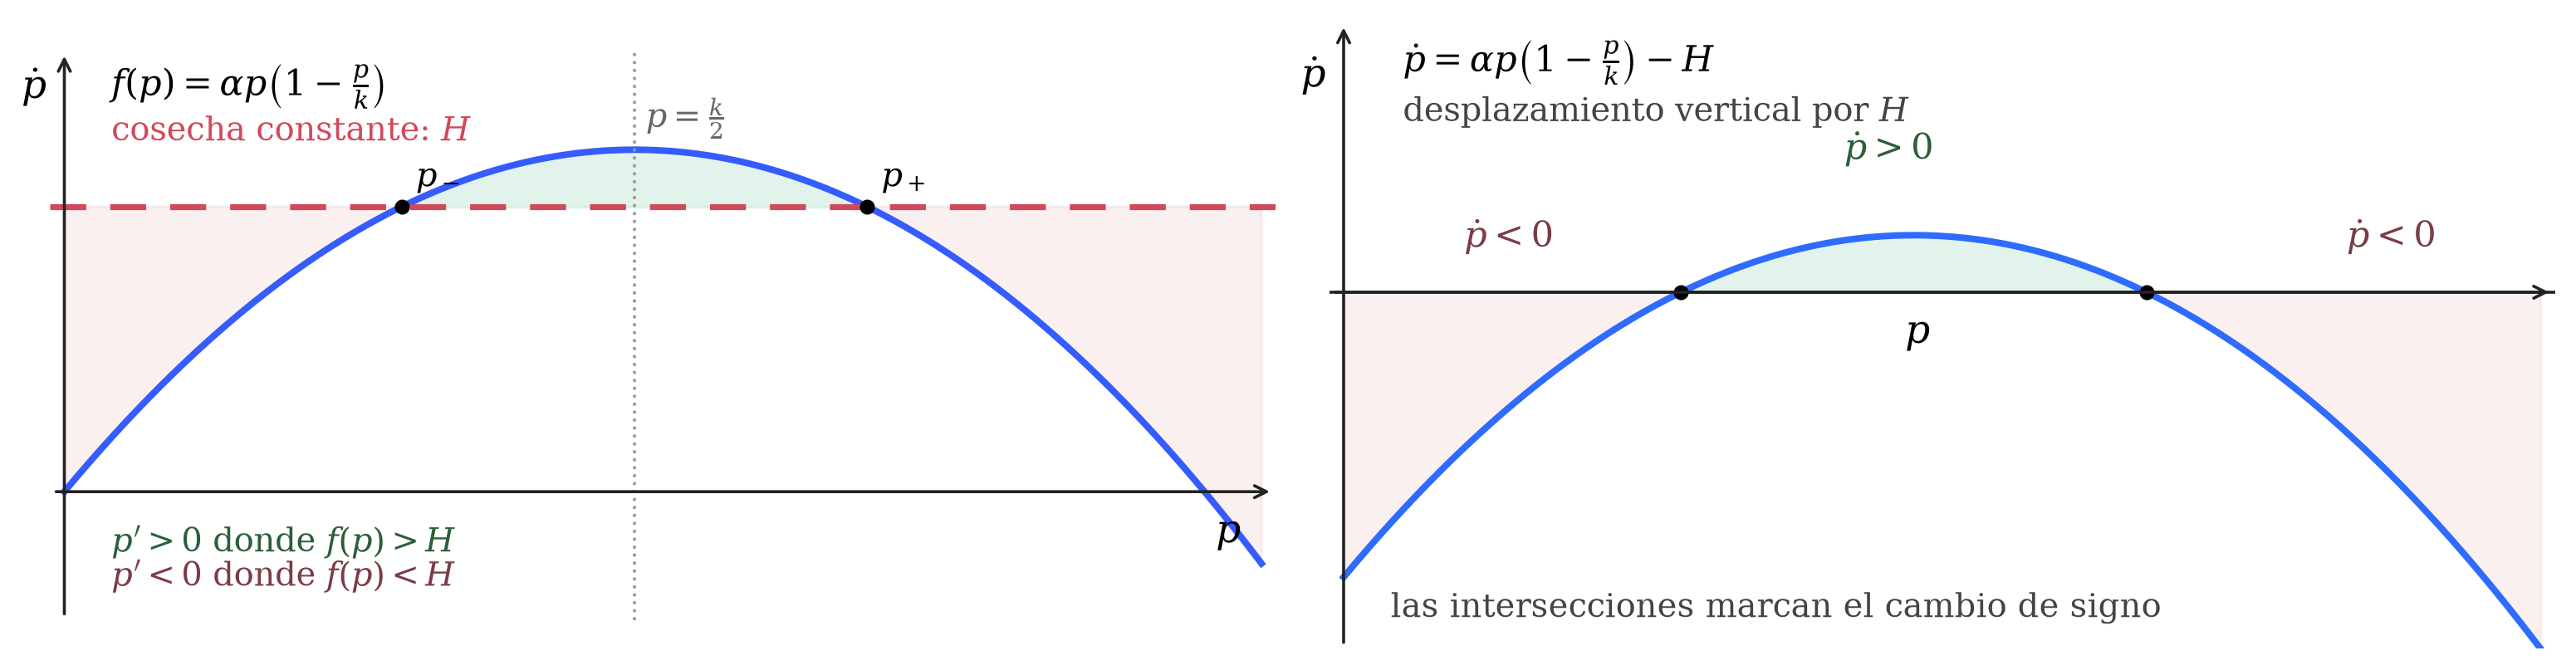
\includegraphics[width=0.92\linewidth]{fig_31_cosecha_logistica.png}
\end{figure}

\newpage
\noindent \textbf{Referencia Nagle:}

\noindent {\scriptsize \url{C:/Users/shint/Music/Proyectos/Apuntes_de_Modelos_Matemáticos_I/Referencias/nagle.md}}

\end{document}

